\label{sec:statistical_framework}

\subsubsection{Fitting framework}

The fitting framework used to parameterise QCD background is based on XML Analytic Workspace Builder~\cite{xmlAnaWSBuilder} (xmlAnaWSBuilder), which employs one-dimensional 
observables to create RooFit~\cite{RooFit} workspaces. The workflow of the framework is summarised in Figure~\ref{fig:xmlAnaWSBuilderworkflow}.

\begin{figure}[htb]
 \centering
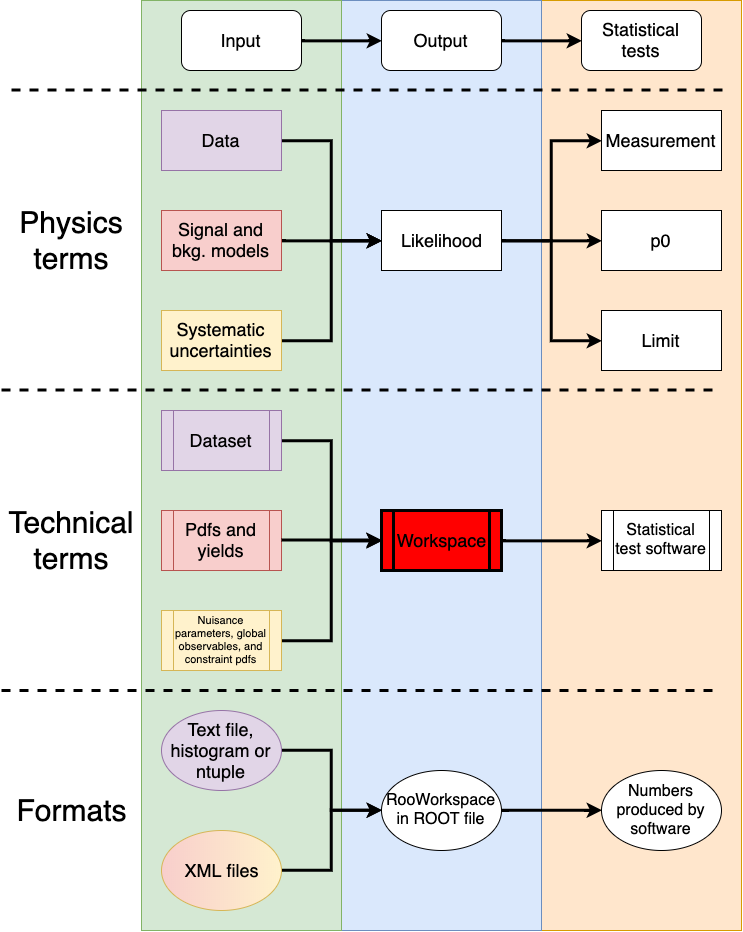
\includegraphics[width=0.75\textwidth]{fig/06-StatisticalFramework/xmlAnaWSBuilder_workflow}
\caption{Workflow of the XmlAnaWSBuilder.  \label{fig:xmlAnaWSBuilderworkflow}}
\end{figure}

The xRooFit framework~\cite{xRooFit} that based on RooFit data fitting package is used for data fitting. Modifications are needed so that it can integrate over binned data, as RooFit evaluates its fit functions using the centre value of each bin rather than the actual average mass in each bin. As a result, significant biases could occur in the fit results~\cite{gligorov2021avoiding}. Recent developments introduce a new class of \texttt{RooBinSamplingPdf} in to RooFit package, which solve such issue.

% in RooFit have created a new class, \texttt{RooBinSamplingPdf}, which can now be used to avoid this problem which is available in a patch to ROOT v6.23~\cite{RooBinSamplingPdf} and built in the v6.24 release. 

%%%%%%%%%%%%%%%%%%%%%%%%%%%%%%%%%%%%%%%%%%%%%%%%%%%%%%%%%%%%%%%%%%%%%% 
%\subsection{Likelihood Definition}
%
%The statistical analysis of the data uses a binned likelihood function~\cite{AlKhoury:2692011} which maximum correspond to the
%best description of data. It is defined as the product over all bins of the Poisson probability to observe $N^{\mathrm{obs}}_i$
%data events given a prediction of $N^{\mathrm{exp}}_i (\mu, \theta)$ events in a certain bin $i$:
%\begin{equation}
%  L (\mu, \theta) = 
%  \prod_{i \in \mathrm{bins}} 
%  \frac{ \left[N^{\mathrm{exp}}_i (\mu,  \theta)\right]^{N^{\mathrm{data}}_i}} {N^{\mathrm{data}}_{i}!}
%  \exp\left[ - N^{\mathrm{exp}}_i (\mu,  \theta) \right]
%%\label{Eq:fitfunction}% uncomment if label used. 
%\end{equation}
%In this likelihood, the number of predicted events is made dependent on two sets of parameters: the signal strength $\mu$ 
%and the  nuisance parameters $\mathbf{\theta} = {\theta_1, \cdots, \theta_l}$, as follows
%
%\begin{equation}
%N^{\mathrm{exp}}_i (\mu,  \theta) = \mu N^{\mathrm{exp}}_{i,\mathrm{sig}}(\mathbf{\theta}) +  N^{\mathrm{exp}}_{i,b}(\mathbf{\theta}).
%%\label{Eq:fitfunction}% uncomment if label used. 
%\end{equation}
%The parameter of interest, $\mu$, is a scale factor for the signal being searched for. The expected number of background 
%events, $N^{\mathrm{exp}}_{i,b}(\mathbf{\theta})$, is measured using functions described in the next sub section where the nuisance
%parameters (NP) are the function parameters. 
%
%The nuisance parameters (NP) $\theta_i$ encode the dependence of the prediction on systematic uncertainties
%into continuous parameters in the likelihood. The prior knowledge on these parameters is reflected by a
%Gaussian penalty term Gauss$(0 | \theta_i,1)$ included in to the likelihood for each NP, rending displacement of these
%parameters depreciated. The parameters $\theta_i$ are therefore expressed in standard deviation in the following.
%It results in a log-normal (normal) dependence of the predicted rates (shapes) on the displayed parameter
%values.
%
%The nominal fit result in terms of $\mu$ and $q_\mu$  is obtained by maximizing the likelihood function with respect
%to all parameters. This is referred to as the maximized log-likelihood value, MLL. The profile likelihood
%ratio test statistic, $q_\mu$ is then constructed as follows:
%\begin{equation}
%q_\mu = 2 \ln \left[ \cal{L}(\mu, \hat{\hat{\mathbf{\theta}}}_\mu) / \cal{L}(\hat{\mu}, \hat{\mathbf{\theta}}_\mu)  \right] 
%\end{equation}
%where $\hat{\mu}$ and $\hat{\mathbf{\theta}}_\mu$ are the parameters that maximise the likelihood 
%(with the constraint $0  \le \hat{\mu} \le \mu$), , and 
%$\hat{\hat{\mathbf{\theta}}}_\mu$ are the nuisance parameter values that maximise the likelihood for a given $\mu$. 
%This test statistic is used to measure the compatibility of the background-only model with the observed data, 
%extracting the local $p_0$
%value, and, if no hint of a signal is found in this procedure, for the derivation of exclusion intervals using
%the \textit{CLs} method.
%%~\cite[Cowan:2010js, Read:2002hq]. 
%%%%%%%%%%%%%%%%%%%%%%%%%%%%%%%%%%%%%%%%%%%%%%%%%%%%%%%%%%%%%%%%%%%%%%%%%%%%%%%
\subsubsection{Statistical method} 

In this analysis, the discriminating variable is set to the dijet invariant mass $m_{jj}$, and the distribution of it is used as  a probability density function (pdf) to build the likelihood function.

\paragraph{Parametric background models}\mbox{}\par
%\subsubsection{Parametric background and signal models}

%The string signals are parameterized as the convolution of an
%exponential, $\lambda_c \exp\left( -\lambda_c m_{jj} \right)$, and a
%Gaussian,  $G(m_{jj};\mu_c,\sigma_c)$, added to an another Gaussian
%$G(m_{jj};m_G,\sigma_G)$. 
%The two terms are weighted by the parameter $a$:

%\begin{eqnarray}
%f_s(m_{jj};\bm{p}_s) & = &
%f_s(m_{jj};a,\lambda_c,\mu_c,\sigma_c,m_G,\sigma_G) = a
%G(m_{jj};m_G,\sigma_G) \nonumber \\ 
%& + & (1 - a) \frac{\lambda_c}{2} \exp \left[
%-\lambda_c \left( m_{jj} - \mu_c - \frac{\lambda_c \sigma_c^2}{2} 
%\right) \right] 
%\mathrm{erfc} \left( 
%\frac{ m_{jj} - \mu_c - \lambda_c\sigma_c^2}{\sqrt{2}\sigma_c}
%\right)\, .
%\end{eqnarray}

%\noindent
%The parameter $a$ is typically fixed, and $\bm{p}_s$ are free parameters
%determined by fitting to MC signal templates. 
%\textit{We may have moved to using the template histograms directly, but
%I keep this parametric description in for a while longer.} 

The distribution of \mjj~of background is parameterized by

\begin{equation}\label{pdfb}
f_b(m_{jj};\bm{p}_b) = f_b(m_{jj};p_1,p_2,p_3,p_4,p_5) = p_1 \left( 1
- \frac{m_{jj}}{\sqrt{s}} \right)^{p_2} \left( \frac{m_{jj}}{\sqrt{s}}
\right)^{p_3 + p_4\ln\left( \frac{m_{jj}}{\sqrt{s}} \right) +  p_5
  \left[ \ln \left( \frac{m_{jj}}{\sqrt{s}} \right) \right]^2}\, .  
\end{equation}

\noindent
where $\bm{p}_b$ are free parameters determined by fitting to data (or 
pseudo data), and $\sqrt{s} = 13$~TeV.
In some cases, $p_5 = 0$ is taken. 
We will assume Equation~(\ref{pdfb}) is normalized to unity as needed.

Given that we are employing a binned likelihood approach and working with histograms, it becomes essential to determine the average count of events in the $i$th bin, arising from both the signal and background contributions:

\begin{eqnarray}
s_i & = & s_\mathrm{tot} \int_{\mathrm{bin}\ i} f_s(m_{jj};\bm{p}_s)
dm_{jj}\, .\\
b_i & = & b_\mathrm{tot} \int_{\mathrm{bin}\ i} f_b(m_{jj};\bm{p}_b) dm_{jj}\, .
\end{eqnarray}

\noindent
where $f_s$ and $f_b$ are pdfs of $m_{jj}$ for the signal and
background, respectively. 
The quantities $s_\mathrm{tot}$ and $b_\mathrm{tot}$ represent the total mean
numbers of signal and background events.
The variable $b_\mathrm{tot}$ is an additional nuisance parameter.
The signal normalization $s_\mathrm{tot}$ is  not treated as a parameter that can be adjusted, but rather is set to the value determined by the nominal signal model. 
The parameter can be expressed as $s_\mathrm{tot} = \sigma L \varepsilon$,
where $\sigma$ is fixed by the model cross section, and $L$ and
$\varepsilon$ represent the nominal luminosity and total acceptance times
efficiency, respectively.


\paragraph{Uncertainties}\mbox{}\par
\label{sec:unc}

In this analysis, there are six sources of systematic uncertainties on the signal studied: 

\begin{description}
\item $\delta L$ an uncertainty on the integrated luminosity of the data
  sample,
\item $\delta\varepsilon$ an uncertainty on the signal efficiency times
  acceptance, 
\item $\delta t$ an uncertainty on the gluon-tag efficiency,
\item $\delta E_\mathrm{JER}$ an uncertainty on the jet energy
  resolution.
\item $\delta E_\mathrm{JES}$ an uncertainty on the jet energy scale.
\item $\delta S$ an uncertainty due to spurious signals.
\end{description}

\noindent
All these uncertainties are treated as shape uncertainties except for
$\delta L$ which is a normalization uncertainty.
These uncertainties are associated to nuisance parameters denoted by
$\alpha_L$,
$\alpha_\varepsilon$, $\alpha_t$, $\alpha_{E_\mathrm{JER}}$,
$\alpha_{E_\mathrm{JES}}$, $\alpha_S$, 
respectively, and the values of the auxiliary measurements by 
$\theta_b$, $\theta_L$, $\theta_\varepsilon$, $\theta_t$,
$\theta_{E_\mathrm{JER}}$, $\theta_{E_\mathrm{JES}}$, $\theta_S$, respectively.


\paragraph{Likelihood function definition}\mbox{}\par

A binned likelihood is used in this analysis. Consider the $m_{jj}$ histogram of $\bm{n} = (n_1, \ldots, n_N)$
events, the likelihood function without uncertainties is built as:
\begin{equation}
\mathcal{L}(\mu;b_\mathrm{tot},\bm{p}_s,\bm{p}_b) = \prod_{i=1}^N \frac{(\mu s_i +
b_i)^{n_i}}{n_i!} e^{-(\mu s_i + b_i)}\, .
\end{equation}
\noindent
where the parameter of interest (POI) $\mu$ is the signal strength
parameter, $b_i$ is the number of background events in the $i$ bin, $s_i$ is the number of signal events in the $i$ bin. Background-only
hypothesis corresponding to $\mu = 0$, whereas nominal signal hypothesis corresponding to $\mu = 1$.

The full likelihood function with uncertainties included is defined as:
%Including uncertainties, the full likelihood function is\footnote{To be succinct, the bin index on the arguments of the functions $N_i$ and $\eta_i$ have been suppressed.}

\begin{eqnarray}
\mathcal{L}(\mu;b_\mathrm{tot},\bm{p}_s,\bm{p}_b,\bm{\alpha}_s)
& = & \prod_{i=1}^N \frac{(\mu^T_i)^{n_i}}{n_i! } e^{-\mu^T_i}
N_i(\alpha_L;\theta_L,\delta_L)
N_i(\alpha_\varepsilon;\theta_\varepsilon,\delta\varepsilon)\nonumber\\
& \cdot &
N_i(\alpha_t;\theta_t,\delta E_t)
N_i(\alpha_{E_\mathrm{JER}};\theta_{E_\mathrm{JER}},\delta E_\mathrm{JER})\\
& \cdot &
N_i(\alpha_{E_\mathrm{JES}};\theta_{E_\mathrm{JES}},\delta E_\mathrm{JES})
N_i(\alpha_S;\theta_S,\delta_S)\, .
\end{eqnarray}

\noindent
where $\mu^T_i$ is the total number of expected event in the $i$ bin, which is
given by:

\begin{equation}
\mu^T_i = \mu s_i 
\eta^L_i(\alpha_L) 
\eta^\varepsilon_i(\alpha_\varepsilon) 
\eta^t_i(\alpha_t)
\eta^{E_\mathrm{JER}}_i (\alpha_{E_\mathrm{JER}})
\eta^{E_\mathrm{JES}}_i (\alpha_{E_\mathrm{JES}}) + b_i \, .
%\eta^b_i(\alpha_b)\, .  
\end{equation}

\noindent
The parameter $\eta^s(\alpha_s)$ are response functions for uncertainty $s$, and
the subsidiary measurements are constrained by the
$N(\alpha;\theta,\delta)$ functions. 

In this analysis, constraint functions are built from standard Gaussians, together with uncertainties that mapped in the response functions. Luminosity uncertainty is fitted by a log-normal response function, the JER and JES uncertainties are given by Gaussian and asymmetric response functions, respectively. For each bin, a vertical interpolation strategy called piece-wise linear method is used independently. In the case of the asymmetric error, the polynomial interpolation and exponential extrapolation method is used.

The parameters $(\mu,N_b,\bm{p}_s,\bm{p}_b,\alpha_L)$ are fixed from the fit to data (pseudo-data) and are common for all bins, whereas parameters
$(\alpha_\varepsilon,\alpha_t,\alpha_{E_\mathrm{JER}},\alpha_{E_\mathrm{JES}},\alpha_S)$ 
are different from bin to bin.

For simplicity in notation, the 18 nuisance parameters are writted as the
vector $\bm{\alpha}$, where six of them have corresponding uncertainties.
The simplified likelihood function is written as:

\begin{equation}
\mathcal{L}(\mu;\bm{\alpha}) = \prod_{i=1}^N
\frac{[\mu^T_i(\mu,\bm{\alpha})]^{n_i}}{n_i!} e^{-\mu^T_i(\mu,\bm{\alpha})}
\prod_{s=1}^6 G_{i,s}(\alpha_s)\, .
\end{equation}

%%%%%%%%%%%%%%%%%%%%%%%%%%%%%%%%%%%%%%%%%%%%%%%%%%%%%%%%%%%%%%%%%%%%%%%%%%%%%%% 
\paragraph{Statistical method}\mbox{}\par

A hypothesis test is used for estimating the compatibility between data and a theoretical hypothesis, where the pseudo datasets are generated according to a given hypothesis, and compared to the tested dataset in terms of a test statistic.

The procedure is demonstrated as follows: first, the agreement between the collected data and the null hypothesis is evaluated through a hypothesis test. The null hypothesis ($\mu = 0$) posits that only the SM background is present. If the data does not exhibit any substantial excess under this hypothesis test, the subsequent step involves establishing an exclusion limit for the targeted signal model on the resonance cross section for \mjj. In this scenario, the hypothesis transforms into a signal + background assumption, leading to the construction of a test statistic based on the signal + background PDF of the discriminating variable.

The statistical measurement's p-value serves as a quantification of the degree of agreement or discrepancy between a hypothesis and the observed data. Mathematically, it represents the integral of the distribution of the test statistic from the value obtained for the dataset in question to infinity. This value characterizes the probability of achieving the observed outcomes assuming the null hypothesis. A lower p-value indicates a higher degree of statistical significance for the observed incompatibility. For instance, if the p-value of the data is below 0.05, it signifies that the likelihood of the observed data aligning with the hypothesis is less than 5\%. This prompts the assertion that the hypothesis can be excluded at the 95\% confidence level (CL).


%%%%%%%%%%%%%%%%%%%%%%%%%%%%%%%%%%%%%%%%%%%%%%%%%%%%%%%%%%%%%%%%%%%%%%%%%%%%%%% 
\paragraph{Test statistic and p-value definitions}\mbox{}\par

A binned maximum likelihood (ML) fitting method is used to extract the signal, together with profile likelihood ratio test statistic. The test statistics used for claiming a positive signal is defined as:

\begin{equation}
q_0 = \left\{ 
\begin{array}{ll}
-2\ln\frac{\mathcal{L}(0,\hat{\hat{\bm\alpha}}(0))}
{\mathcal{L}(\hat{\mu},\hat{\bm\alpha})} 
& \hat{\mu} \ge 0\, ,\\ 
0 & \hat{\mu} < 0\, .
\end{array}
\right.
\end{equation}

\noindent
and the test statistic used for evaluating the upper limits is given as:

\begin{equation}
\tilde{q}_\mu = \left\{ 
\begin{array}{ll}
-2\ln\frac{\mathcal{L}(\mu,\hat{\hat{\bm\alpha}}(\mu))}
{\mathcal{L}(0,\hat{\hat{\bm\alpha}}(0)}
& \hat{\mu} < \mu\, ,\\ 
-2\ln\frac{\mathcal{L}(\mu,\hat{\hat{\bm\alpha}}(\mu))}
{\mathcal{L}(\hat{\mu},\hat{\bm\alpha})} 
& 0 \le \hat{\mu} \le \mu\, ,\\ 
0 & \hat{\mu} > \mu\, .
\end{array}
\right.
\end{equation}

\noindent
where the parameter $\mu$ represents the signal strength associated with the hypothesis being tested. The maximum likelihood (ML) estimators that optimize the likelihood function $\mathcal{L}$ without constraints are referred to as $\hat{\mu}$ for the signal strength and $\hat{\bm\alpha}$ for the other parameters. The parameter $\hat{\hat{\bm\alpha}}$ represents the conditional ML estimator of $\bm\alpha$ that maximizes $\mathcal{L}$ while considering a specific value of $\mu$.

The p-value corresponding to the background-only hypothesis is expressed as:
\begin{equation}
p_0 = \int_{q_{0,\mathrm{obs}}}^\infty
f(q_0|0) dq_0\, .
\end{equation}

The values of $\tilde{q}_\mu$ are calculated for different values of $\mu$ by fitting a dataset where the pseudo data is represented by $\mu^\prime$. This calculation of $\tilde{q}_\mu$ is conducted for each pseudo dataset at various selected signal mass points, resulting in a distribution of $\tilde{q}_\mu$ denoted as $f(\tilde{q}_\mu|\mu = \mu^\prime)$. As a result, a p-value for the tested dataset is determined based on this distribution:

\begin{equation}
p_{\mu^\prime} = \int_{\tilde{q}^\prime_{\mu,\mathrm{obs}}}^\infty
f(\tilde{q}_\mu|\mu = \mu^\prime) dq_\mu\, ,
\end{equation}

\noindent
the term $\tilde{q}_{\mu^\prime,\mathrm{obs}}$ represents the computed value of the test statistic based on the dataset being tested. These p-values are also referred to as $p_{s+b}$, which signifies that they are associated with the signal plus background hypothesis.

%%%%%%%%%%%%%%%%%%%%%%%%%%%%%%%%%%%%%%%%%%%%%%%%%%%%%%%%%%%%%%%%%%%%%%%%%%%%%%% 
\paragraph{Generation of pseudo-data}\mbox{}\par

The PDF of a certain model is used for generating the pseudo datasets. Signal + background pseudo datasets are utilized to estimate the observed confidence level (CL) of a signal + background hypothesis, while background-only pseudo datasets are employed for expected CL estimations.

During the generation of pseudo datasets, all parameters in the PDF are set to their nominal values. The expected event counts in each bin follow a Poisson distribution. Nuisance parameters (NPs), which represent systematic uncertainties, are treated according to the "unconditional ensemble" approach: for each pseudo dataset, the values of $\alpha_i$ (associated with the NPs) are drawn from their respective constraint terms, and these values are used in both the likelihood $\mathcal{L}$ and the computation of $\tilde{q}_\mu$.




%%%%%%%%%%%%%%%%%%%%%%%%%%%%%%%%%%%%%%%%%%%%%%%%%%%%%%%%%%%%%%%%%%%%%%%%%%%%%%% 
\paragraph{Definition of exclusion limit}\mbox{}\par

The data is interpreted by the modified frequentest method ($CL_S$ method), where p-value is modified to take into account
downward background fluctuations and quoted as
$CL_s$. The definition of $CL_s$ is:


\begin{equation}
CL_s = \frac{p_{s+b}}{1-p_b}\, ,
\end{equation}

\noindent
where $p_{b(s+b)}$ is the integrated value of the background-only (signal + background) distribution
from zero to $\tilde{q}_\mu^\mathrm{obs}$.
Thus $1 - p_b$ is also referred to as the confidence level of the
background-only hypothesis ($CL_b$). The $CL_s$ limit claims exclusion at 95\% CL when $CL_s = 0.05$.
%%%%%%%%%%%%%%%%%%%%%%%%%%%%%%%%%%%%%%%%%%%%%%%%%%%%%%%%%%%%%%%%%%%%%%%%%%%%%%% 
\paragraph{Implementation}\mbox{}\par
%The statistical approach employed in this analysis differs slightly from previous dijet analyses and aligns with the current trigger-level analysis. In previous approaches, a background model devoid of NPs was fitted to the data, and the resulting background fit parameters were employed (and held constant) in subsequent likelihood fits involving nuisance parameters. However,
In this analysis, the background fit parameters are treated as unconstrained NPs within the complete likelihood framework used in all fits.
To create the RooFit workspaces, the XML Analytic Workspace Builder is utilized. The xRooFit tool processes these workspaces and performs operations like setting limits, among others, using classes from the RooFit and RooStats libraries.
%%%%%%%%%%%%%%%%%%%%%%%%%%%%%%%%%%%%%%%%%%%%%%%%%%%%%%%%%%%%%%%%%%%%%%%%%%%%%%% 

\subsubsection{Background estimation}

In the resonant search the SM background of the \mjj\ spectrum is established through a functional fitting procedure applied to the data. Refs.~\cite{Bagnaia:1984ip,PhysRevD.79.112002,EXOT-2010-01,CMS-EXO-10-010,EXOT-2010-07,EXOT-2013-11})
have found that a parametric function of the form
\begin{equation}
  f(x) = p_1 (1 - x)^{p_2} x^{p_3 + p_4\ln x + p_5 (\ln x)^2}.
\label{Eq:fitfunction}% uncomment if label used. 
\end{equation}
where $x \equiv \mjj /\sqrt{s}$, accurately describes dijet mass distribution predicted by leading and next-to-leading-order 
QCD Monte Carlo. In the ATLAS Run~2 analysis with \integLumi\ of data  \cite{EXOT-2019-03,Nishu:2646455}, the four parameter 
version of the function ($p_5 = 0$) was found to sufficiently described the data.  
The introduction of  gluon tagging may require more  parameters to properly describe the full invariant mass spectrum, where no significant deviation is observed, as shown in Figure~\ref{fig:5p}.
 \begin{figure}[!htb]
	   \centering
	   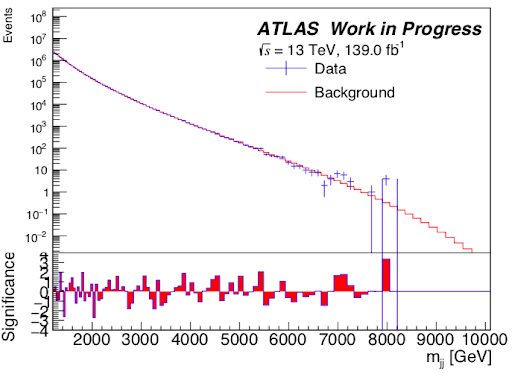
\includegraphics[width=0.45\textwidth]{fig/5presult.png}
	   \caption{\mjj\ background fit.}
		   \label{fig:5p}}
 \end{figure}

%To avoid introducing any potential bias due to the selection of a specific background function, an alternative functional form is employed. This alternative form is inspired by the one used by the UA2 experiment \cite{Alitti:1990kw, Alitti:1993pn} when observing the decay of $W$ and $Z$ bosons into two jets, followed by a subsequent search.
%\begin{equation}
%  f(x) = p_1 x^{p_2} \exp\left({p_3 x + p_4  x^2 }\right).
%%\label{Eq:fitfunction2}% uncomment if label used. 
%\end{equation}

\subsubsection{Analysis strategy}

The analysis begins with the utilization of skimmed ntuples, which are the result of applying the event selection criteria outlined in Section~\ref{sec:analysiscuts}. These ntuples serve as the basis for generating pseudo-data using the background-only model. Subsequently, a 4-parameter ($p_5$ = 0) fit function described by Equation~\ref{Eq:fitfunction} is employed to fit this pseudo-data. The fit to the data is deemed satisfactory if it meets the following criterion:

\begin{itemize}
	\item Global $\chi^2$ $p$-value > 0.05
\end{itemize}

If the conditions mentioned above are satisfied, the background is chosen for the purpose of upper limit estimations. Conversely, if the criteria are not met, the 5-parameter version of Equation~\ref{Eq:fitfunction} is employed for background fitting and is subjected to the same selection criterion. If the fit using the 5-parameter function also fails to meet the criteria, the analysis reduces the range of the window and repeats the fitting process with the 5-parameter function to see if a satisfactory fit can be achieved. If this attempt still does not meet the criteria, the analysis switches to an alternative option for generating pseudo-data. Once a fit satisfying the criteria is obtained, the fit function undergoes various validation tests to ensure the appropriateness of the fit strategy. The flowchart of Figure~\ref{eflow} shows the analysis strategy.

 
\begin{figure}[htb]
\centering
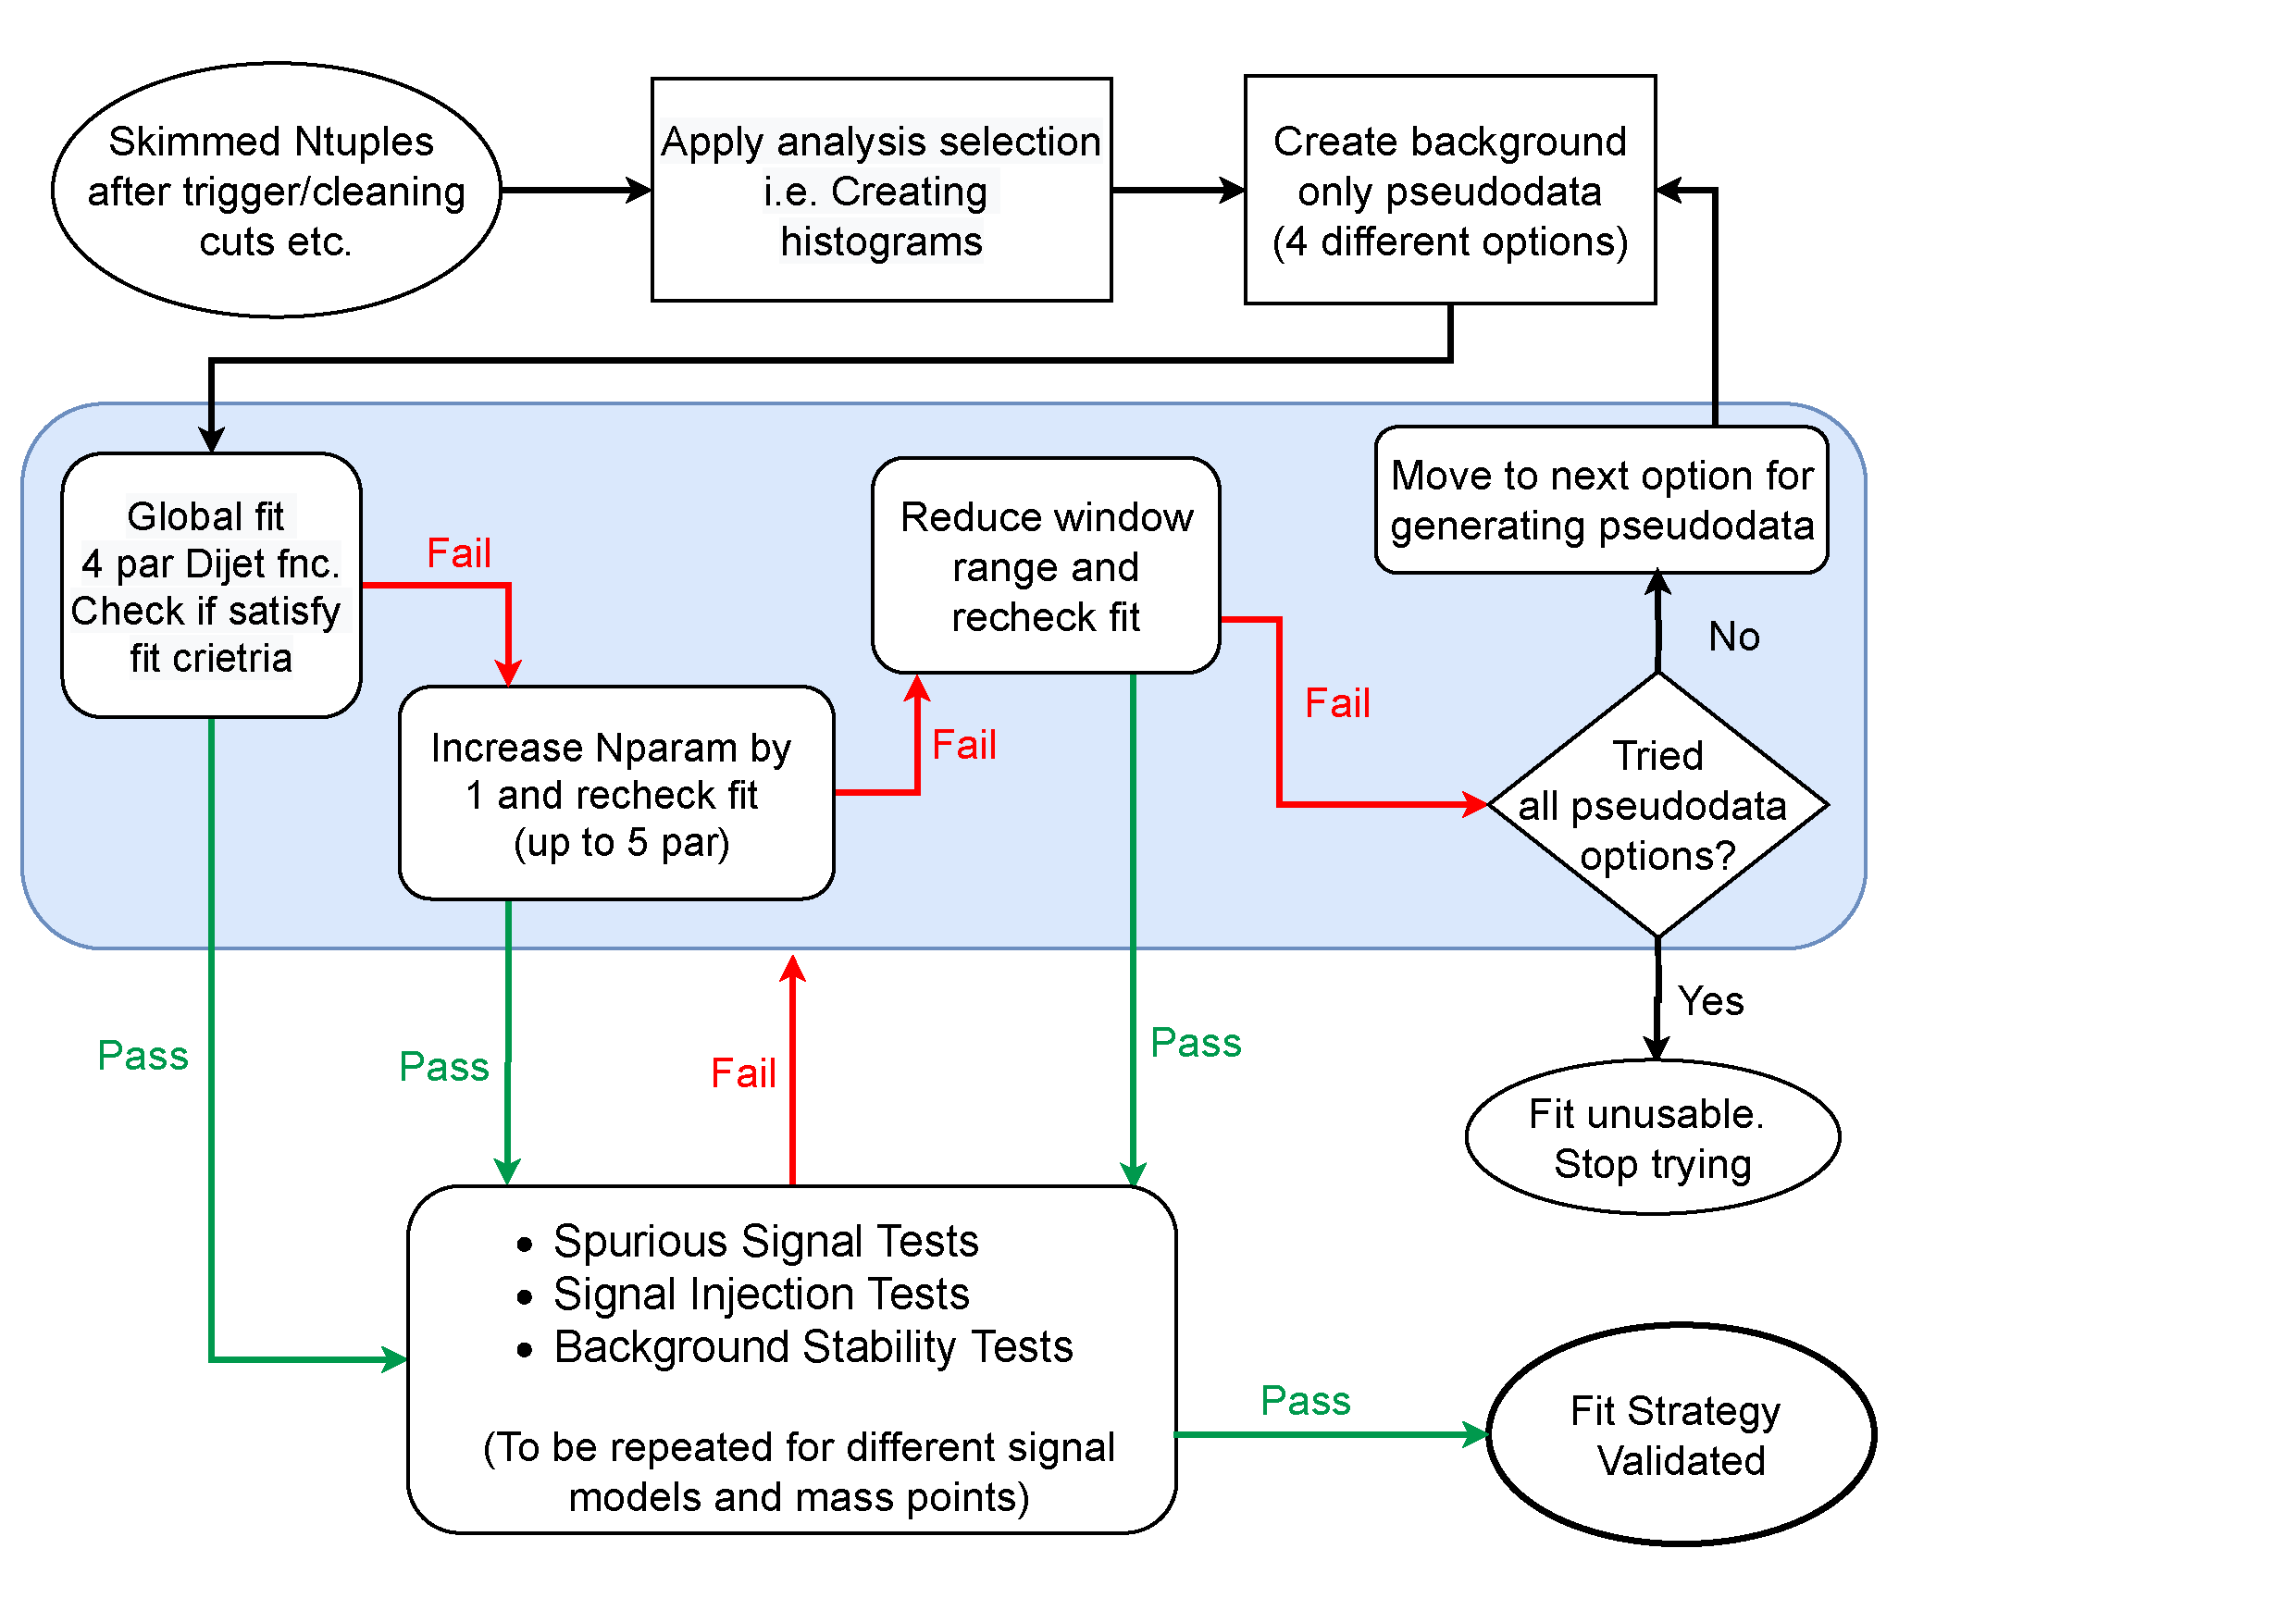
\includegraphics[width=1.1\textwidth]{fig/flowcharts/QGDijet-FlowChart-30March}
\caption{Analysis top-level flowchart.
\label{eflow}}
\end{figure}
%
%\subsubsection{Pseudo-data generation}
%\label{section:pseudo-data}
%
%The analysis strategy is shown in the flowchart in Figure~\ref{eflow}. This section shows the multiple possible options for
%creating background only pseudo-data mentioned in the flowchart. Four options have been discussed here, two of them are
%based on the untagged dijet data used in the already published inclusive dijet Run-2 search~\cite{Nishu:2646455} and the other two are entirely based on Monte Carlo.
%For the ones based on the untagged dijet data, the analysis selection for the current iteration of the analysis
%was compared to the previous one and it was confirmed that we are using a subset of the standard inclusive dijet selection from
%previous iteration with an additional cut on $\eta$ and qg tagging specific cuts.
%
%\paragraph{Option 1\\}
%The first option here starts with using untagged dijet data using the selection for the current round of analysis.
%This untagged dijet data is to be fitted with 5-parameter global fit
%function. Then the fraction of events passing 1 or 2 gluon tag selection are then computed from MC. These fractions are then smoothed to
%get rid of any statistical fluctuations. These smoothed tagging effciencies are then applied to the fitted untagged data to obtain the pseudo-data.
%%A pictorial representation of this can be seen in Figure~\ref{}.
%
%\paragraph{Option 2\\}
%This also starts with using untagged dijet data using the selection for the current round of analysis.
%This untagged dijet data is to be fitted with a 5-parameter global fit function. To obtain the fraction of events
%passing 1 or 2 gluon selection, an ABCD method is to be used. 
%In this method, the data is categorized into four regions by two not strongly correlated variables, the \ystar\
%and gluon tagging. The four regions are defined below:
%
%\begin{itemize}
%\item \texttt{Region A:} Two jets with $|\ystar| > 0.8$, two(>=one) of them are gluon tagged
%\item \texttt{Region B:} Two jets with $|\ystar| < 0.8$, two(>=one) of them are gluon tagged
%\item \texttt{Region C:} Two jets with $|\ystar| > 0.8$
%\item \texttt{Region D:} Two jets with $|\ystar| < 0.8$
%\end{itemize}
%
%By inverting the \ystar\ criterion in region A and C, the signal contamination can be ignored. Data in region B
%(the signal region) can be modeled by the following formula:
%
%\begin{equation}
%N_{B} = N_{D}\epsilon\, ,
%\end{equation}
%
%where $N_{B}$($N_{D}$) is the yield in region B(D) and $\epsilon$ is the per event gluon tagging
%efficiency obtained via region A and C. These are then smoothed to get rid of the
%statistical fluctuations, and applied to the fitted untagged data to obtain the pseudo-data.
%%A pictorial representation of this can be seen in Figure~\ref{}.
%
%\paragraph{Option 3\\}
%This option relies entirely on Monte Carlo samples. First the inclusive selection (without q/g tagging specific cuts)
%is applied to the MC. The fraction of events passing 1 and 2 gluon selection are obtained from the MC sample as well. These
%fractions are then smoothed as in the previous two options, and then applied to the untagged dijet MC to obtain the pseudo-data.
%%A pictorial representation of this can be seen in Figure~\ref{}.
%
%\paragraph{Option 4\\}
%This option uses the MC with all selection cuts applied including the q/g tagging selection.
%A smoothing is applied to this spectrum and this would need to be revisited
%in case the fitting fails to make sure our pseudo-data is always $N_{param+1}$.
%%A pictorial representation of this can be seen in Figure~\ref{}.
%This option suffers from lack of statistics, along with being entirely based on MC and is thus of least preference.
%
%\subsubsection{Pseudo-data for 1 gluon and 2 gluon tag categories}
%This section give details about the pseudo-data used for the fit validation studies.
%We have used Option 1 to create this pseudo-data as discussed in previous section. The $m_{jj}$ spectrum was
%obtained using full Run-2 data with the following selection cuts:
%
%\begin{itemize}
%\item Trigger: Passes the lowest unprescaled single-jet trigger, HLT\_j420
%\item Jet preselecton: Leading jet $\pt\ge 380\,\GeV$ and jet multiplicity $\ge 2$
%\item $|\Delta\phi|$ between two jets: $|\Delta\phi| > 1.0$
%\item $|\ystar|$ between two jets: $|\ystar|<0.8$
%\item \mjj\ $>$  1200\,\GeV
%\item $|\eta|$ for both jets: Jets must be fully within the tracking acceptance ($|\eta|<2.1$)
%\end{itemize}
%
%This spectrum is then fitted with 5 parameter global fit function using Minuit2. Figure~\ref{fig:mjjFit_ystar0p8} shows the results of the fit.
%To obtain the fraction of events passing one gluon tag selection from the inclusive
%spectrum, the same selection as mentioned above has been applied to the Pythia dijet MC samples.
%Figure~\ref{fig:fraction_1gtag_unsmooth} shows these fractions for the one gluon tag category.
%
% \begin{figure}[!htb]
%   \centering
%   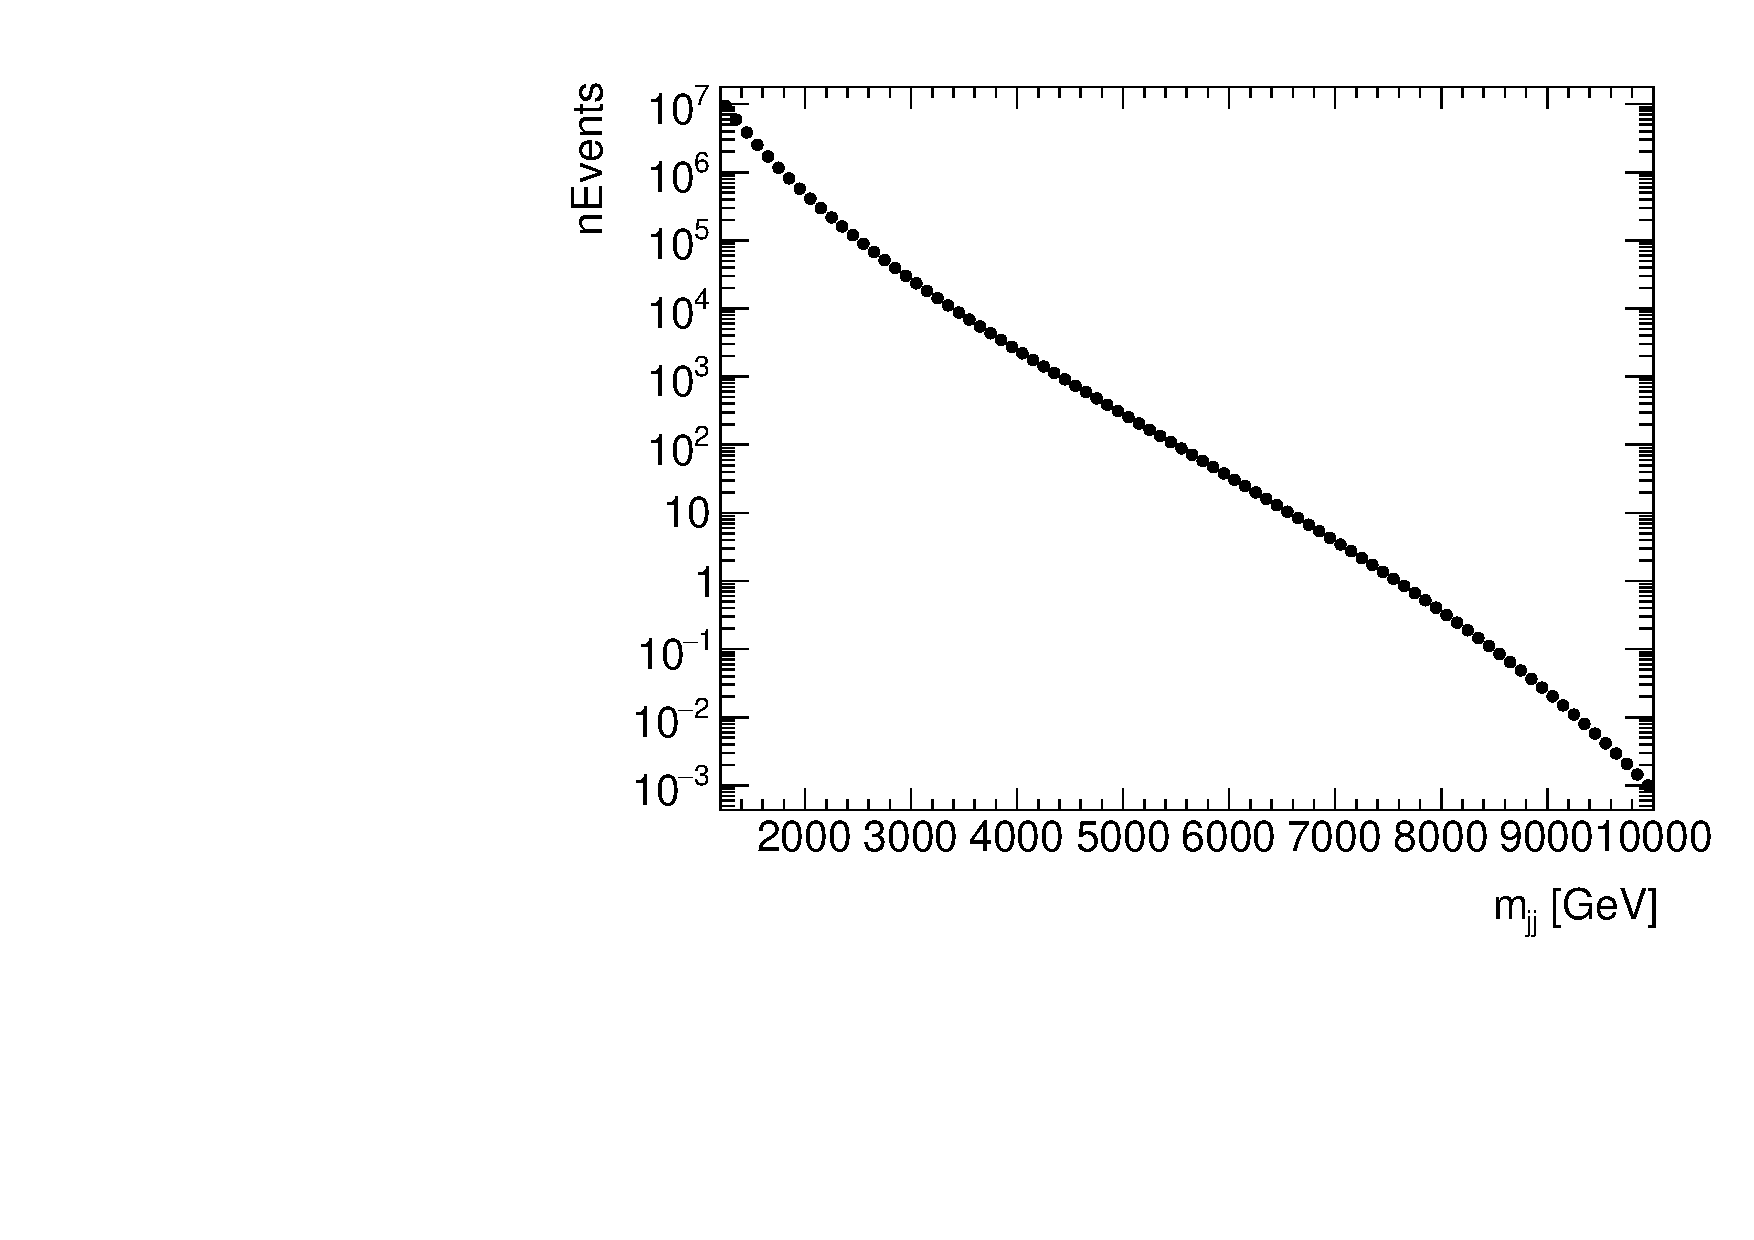
\includegraphics[width=0.45\textwidth]{fig/pseudodata/FittedMjj_UntaggedData_yStar0p8}
%   \caption{Untagged dijet spectrum with $|\ystar|<0.8$ using full Run-2 data fitted with 5-parameter global fit function.
%   \label{fig:mjjFit_ystar0p8}}
% \end{figure}
%
% \begin{figure}[!htb]
%   \centering
%   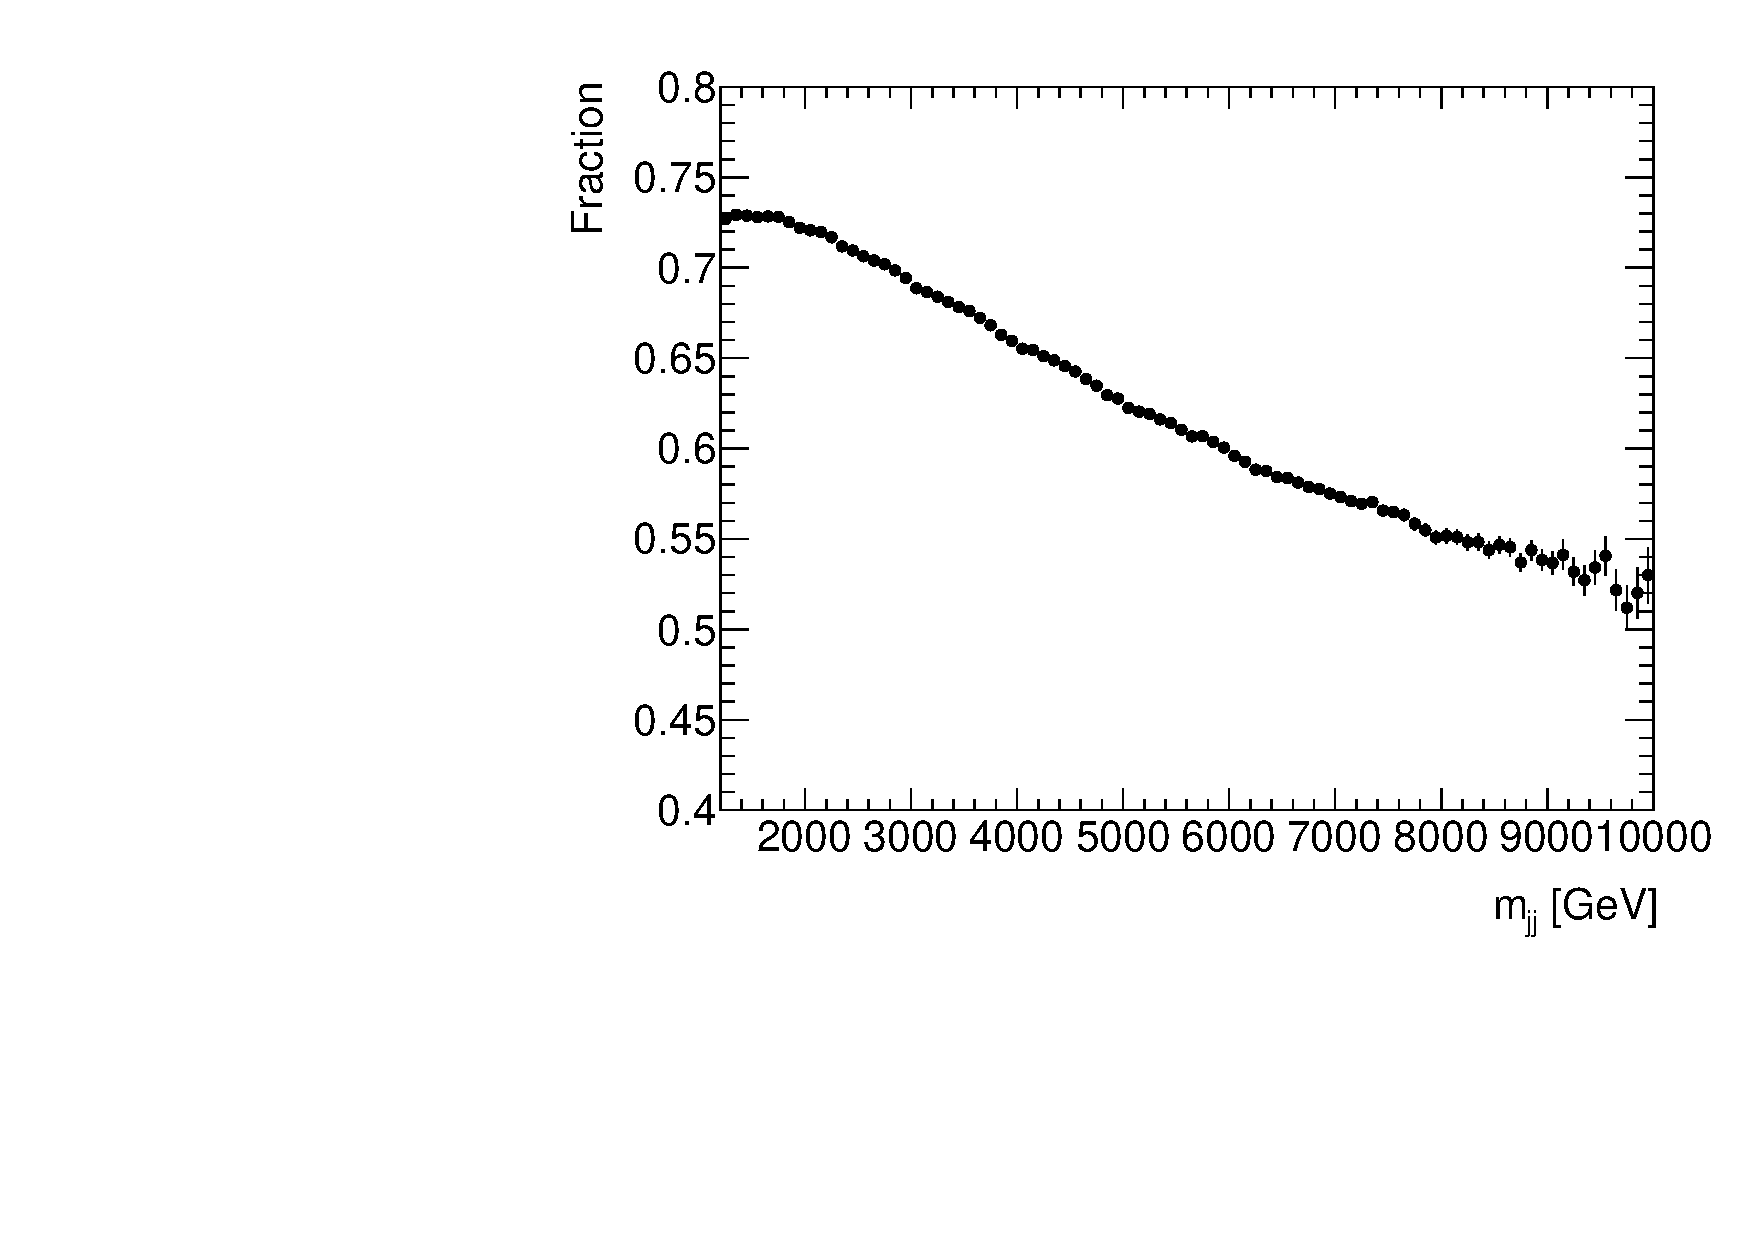
\includegraphics[width=0.45\textwidth]{fig/pseudodata/FractionUnsmooth_1gtag_yStar0p8}
%   \caption{Fraction of events passing 1 gluon tag selection.
%   \label{fig:fraction_1gtag_unsmooth}}
% \end{figure}
%
%
%To smooth these fractions, a smoothing based on Friedman's SuperSmoother
%%: https://github.com/jakevdp/supersmoother 
%has been used. Supersmoother is a non-parametric locally-linear smoother in which the size of the local neighborhood is tuned
%to the characteristics of the data. The degree of smoothing can be tuned with the bass enhancement feature.
%This is a number (alpha) which lies between 0 and 10, with 10 being a much smoother curve. Different options were tried
%for this smoothing parameter, with the ratios to the unsmoothened fractions obtained. Figure~\ref{fig:smoothFractions_1gtag} shows
%the smoothed fractions along with the comparisons to the unsmoothed fractions. It is seen that a larger smoothing
%parameter gives a smoother curve but leads to some shape differences as seen in the ratio plots, so a compromise between the two
%has been used. Some tests with BumpHunter were also performed to evaluate the differences between these different
%smoothing parameters. The very high values of smoothing parameter (9,10) were avoided because of the change in the
%shape of the spectrum based on those tests. For the 1 gluon tag category, smoothing parameter 7 (Figure.~\ref{fig:smoothFractions_1gtag}(b)) was used. 
%
%\begin{figure}[htbp]
%        \centering
%        \subfloat[Smoothing parameter 1]{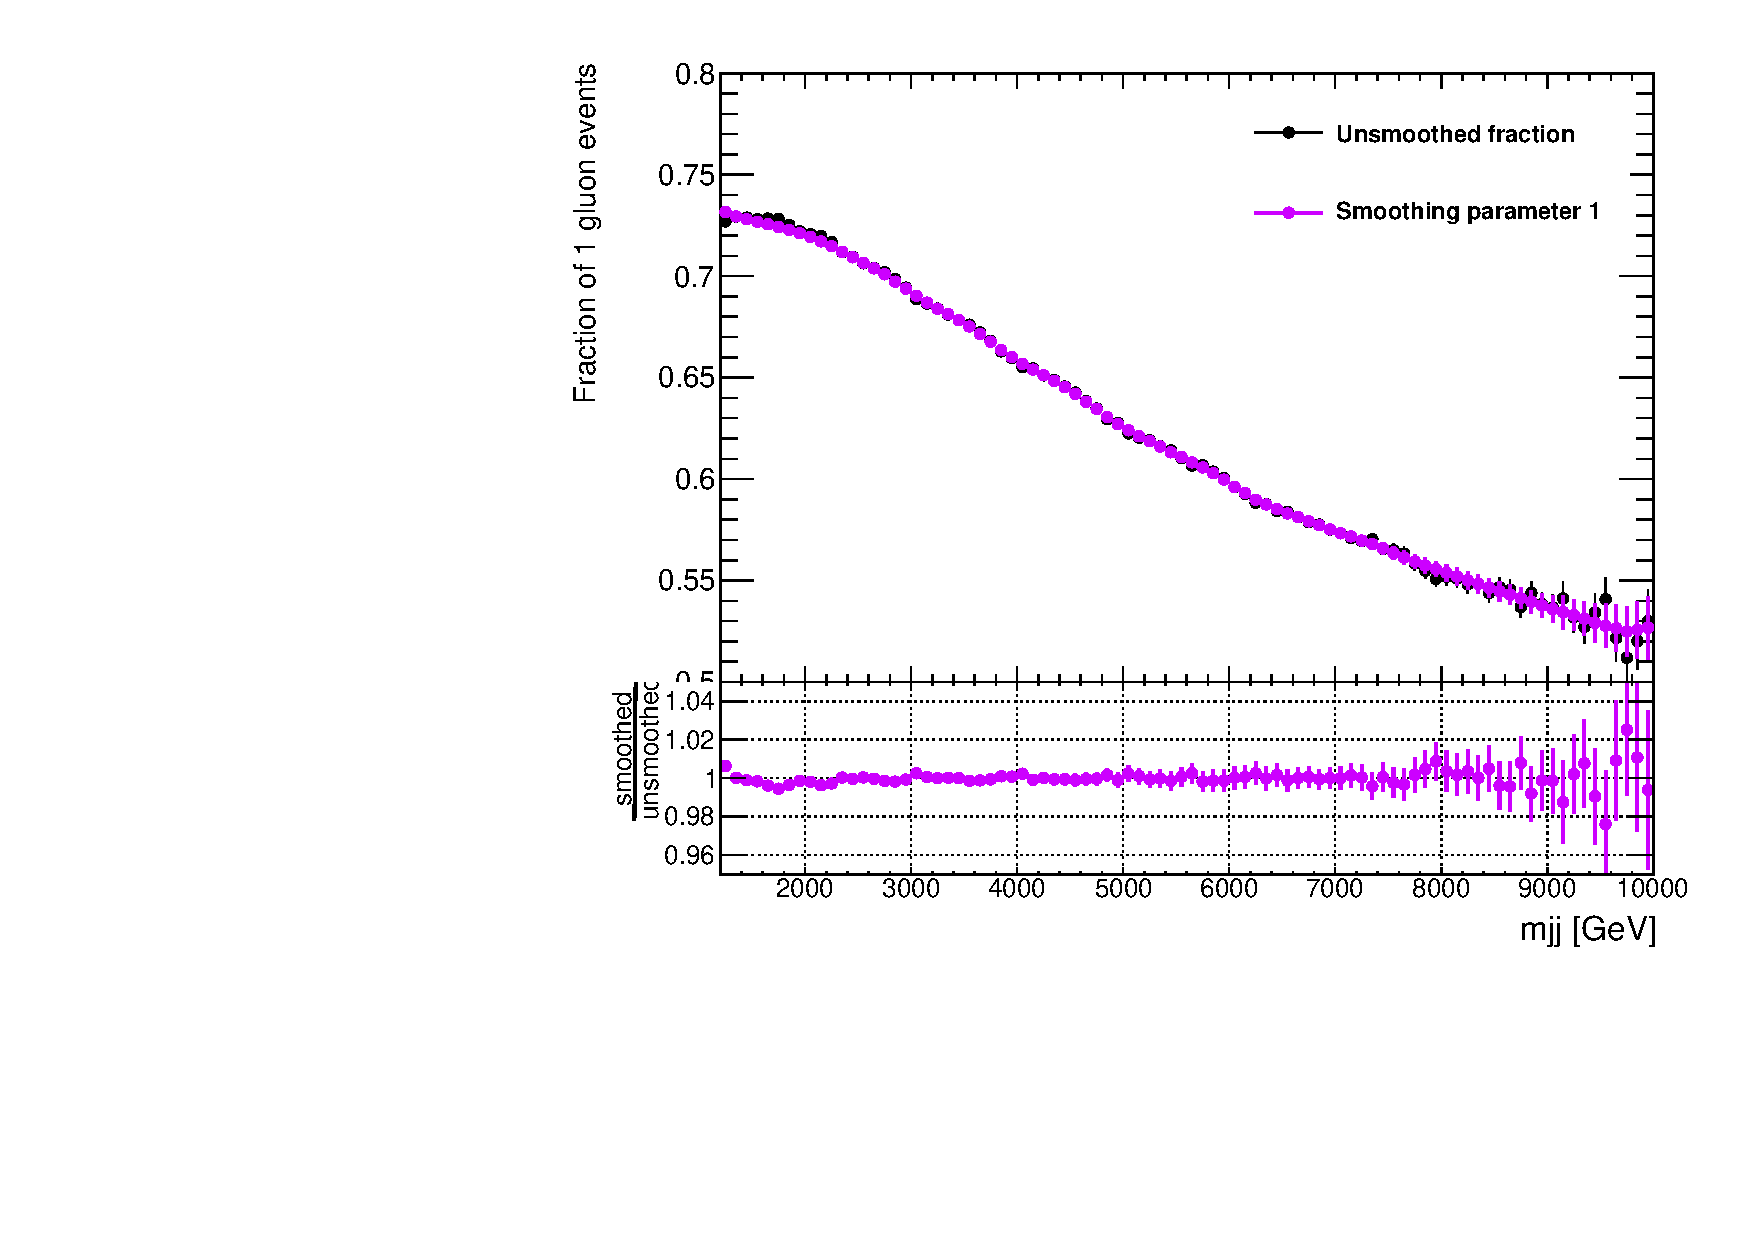
\includegraphics[width=0.48\columnwidth]{fig/pseudodata/Fraction_1gluon_Alpha1to0}}
%        \subfloat[Smoothing parameter 7]{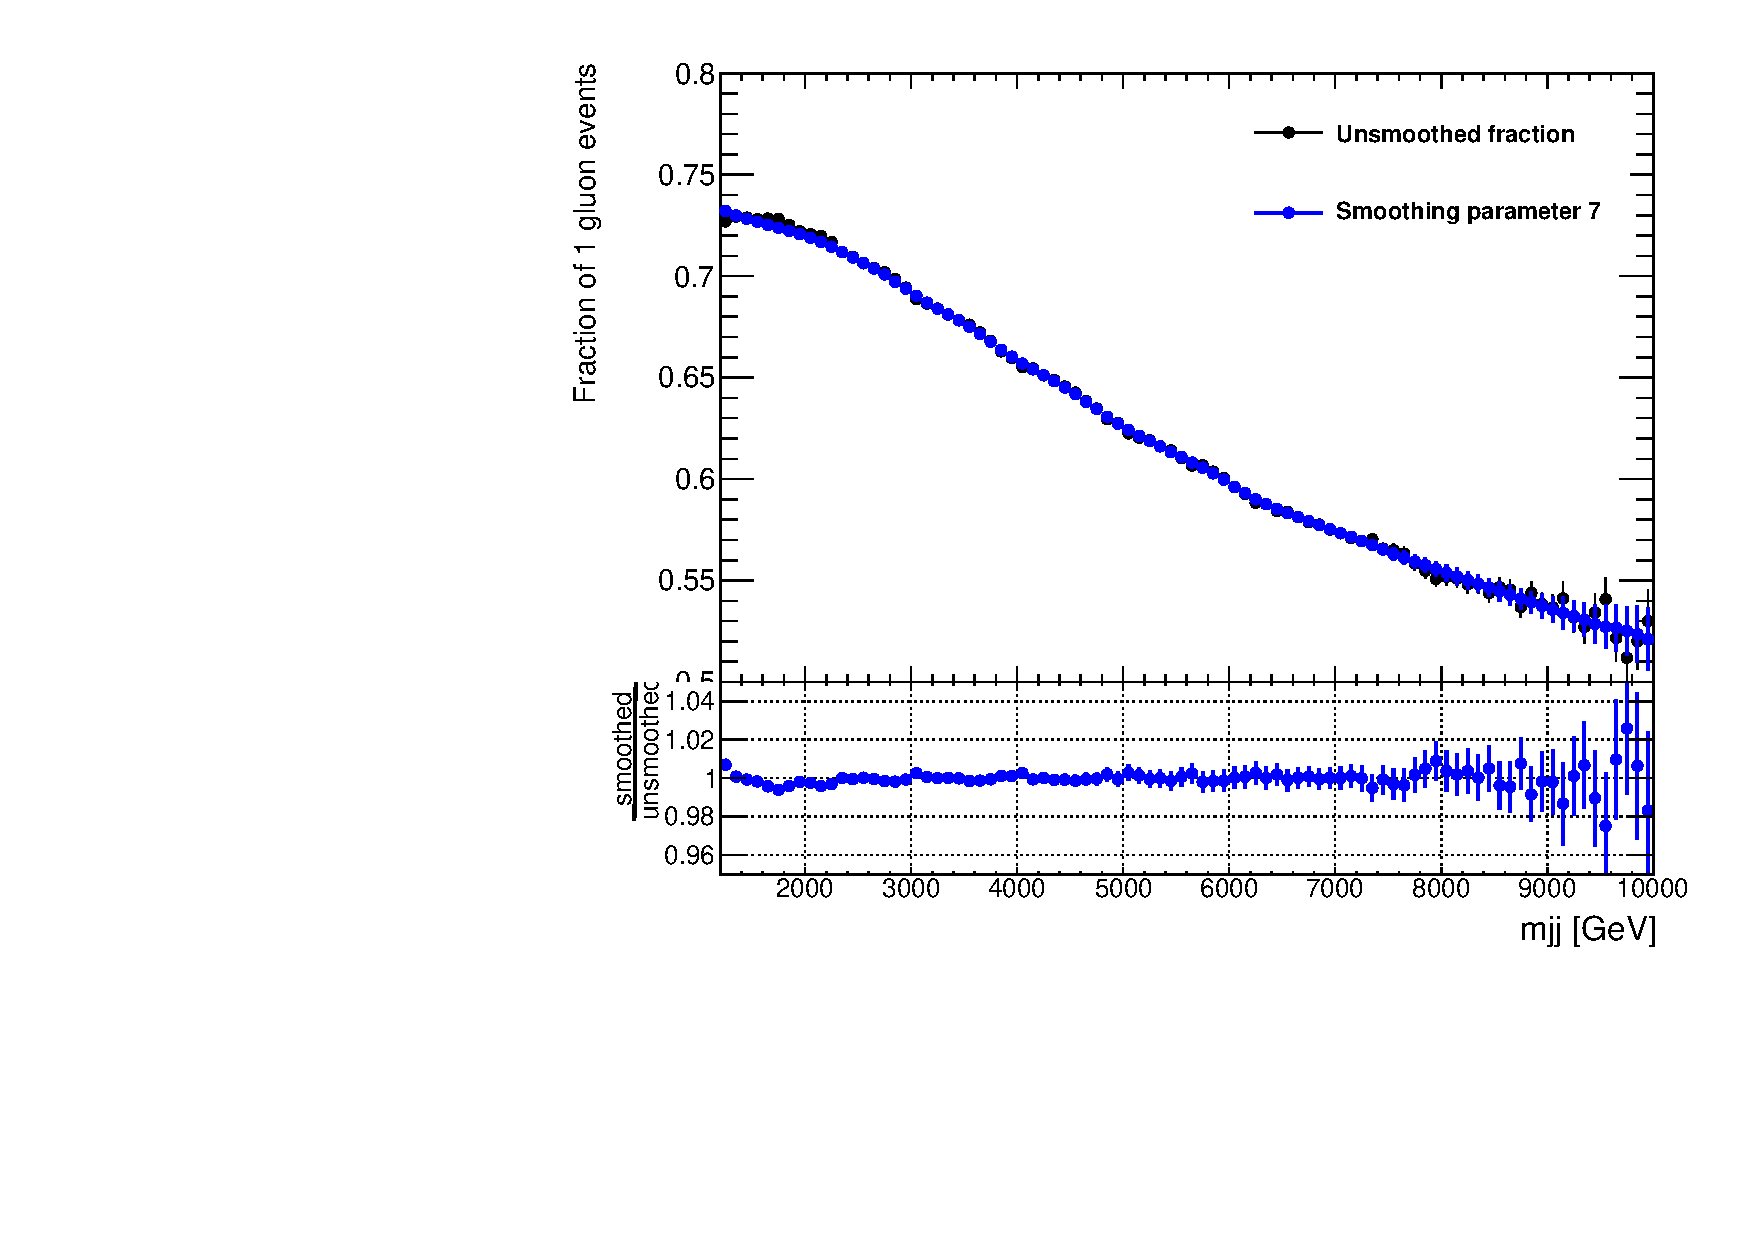
\includegraphics[width=0.48\columnwidth]{fig/pseudodata/Fraction_1gluon_Alpha7to0}}
%        \\
%        \subfloat[Smoothing parameter 8]{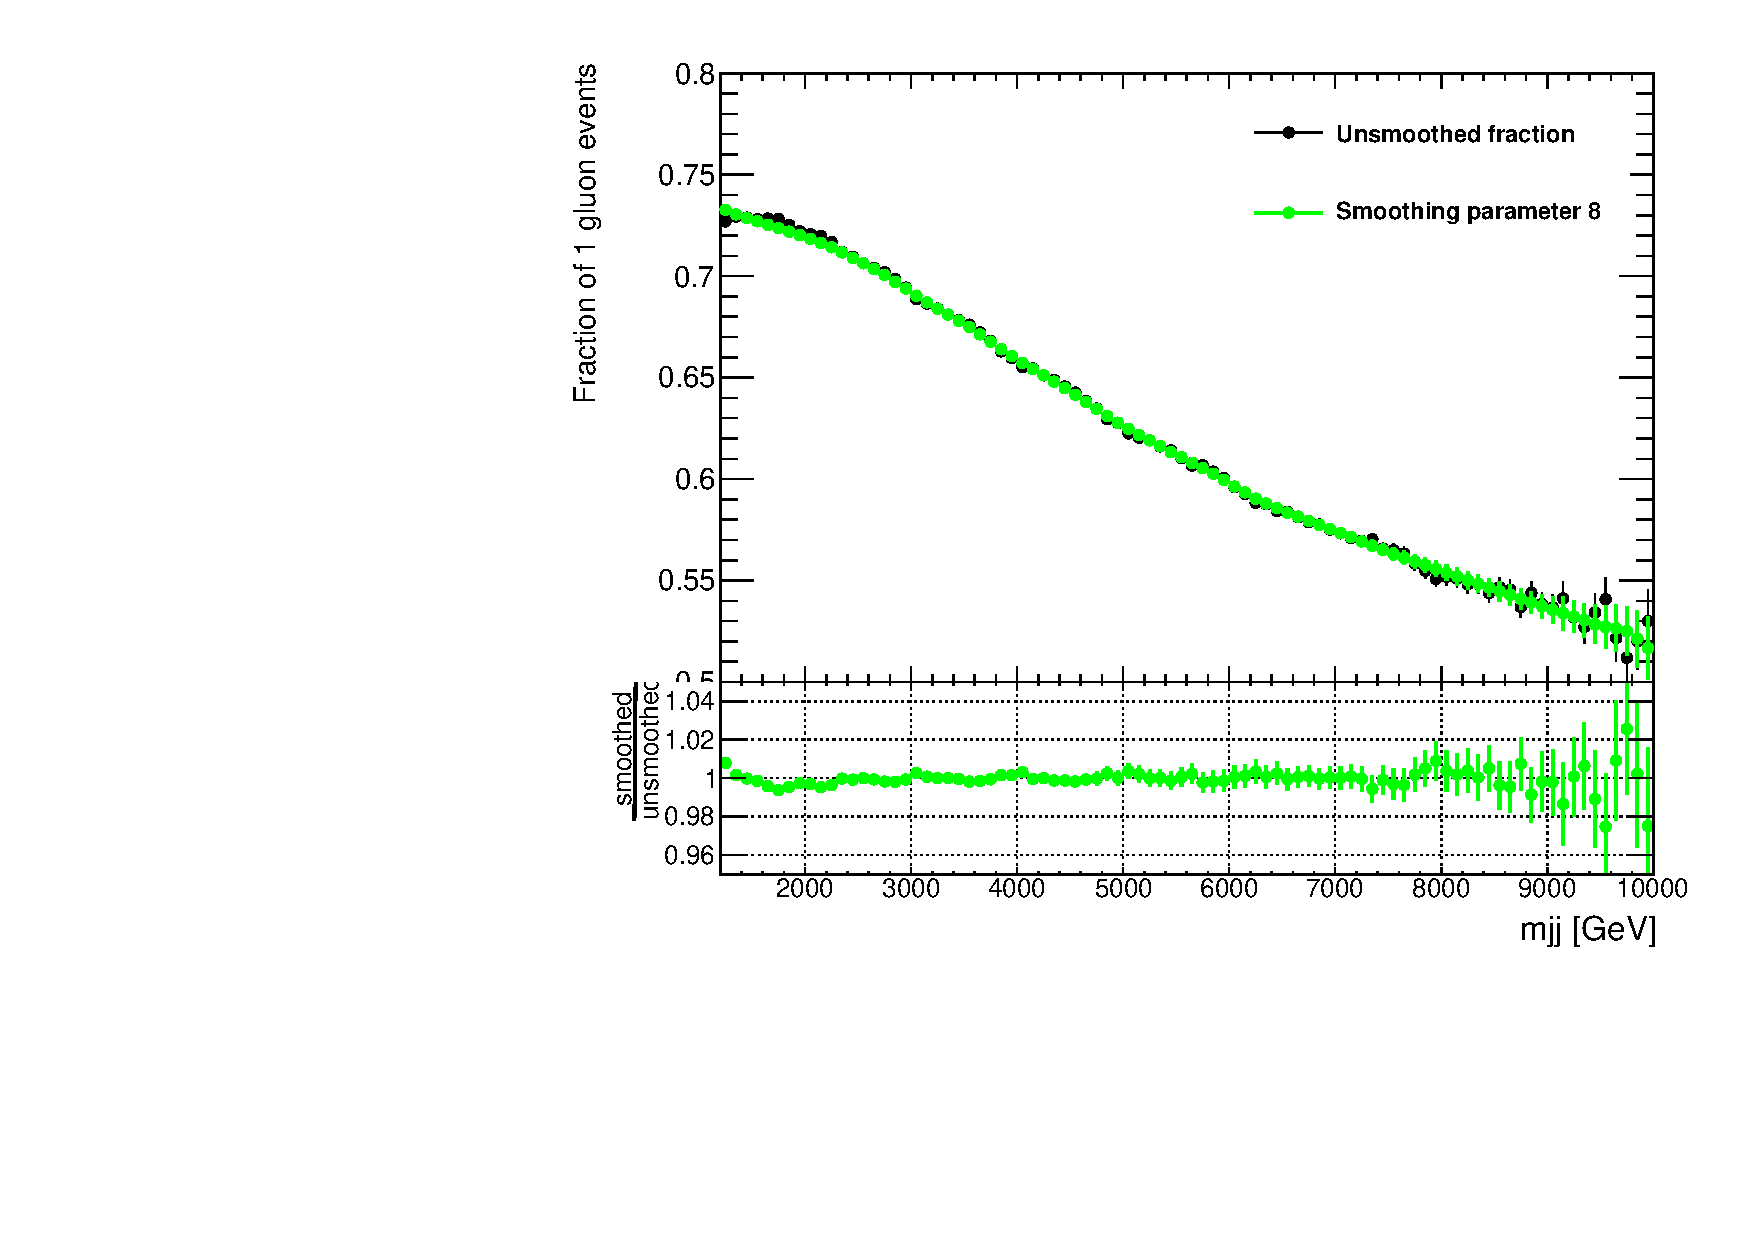
\includegraphics[width=0.48\columnwidth]{fig/pseudodata/Fraction_1gluon_Alpha8to0}}
%        \subfloat[Smoothing parameter 10]{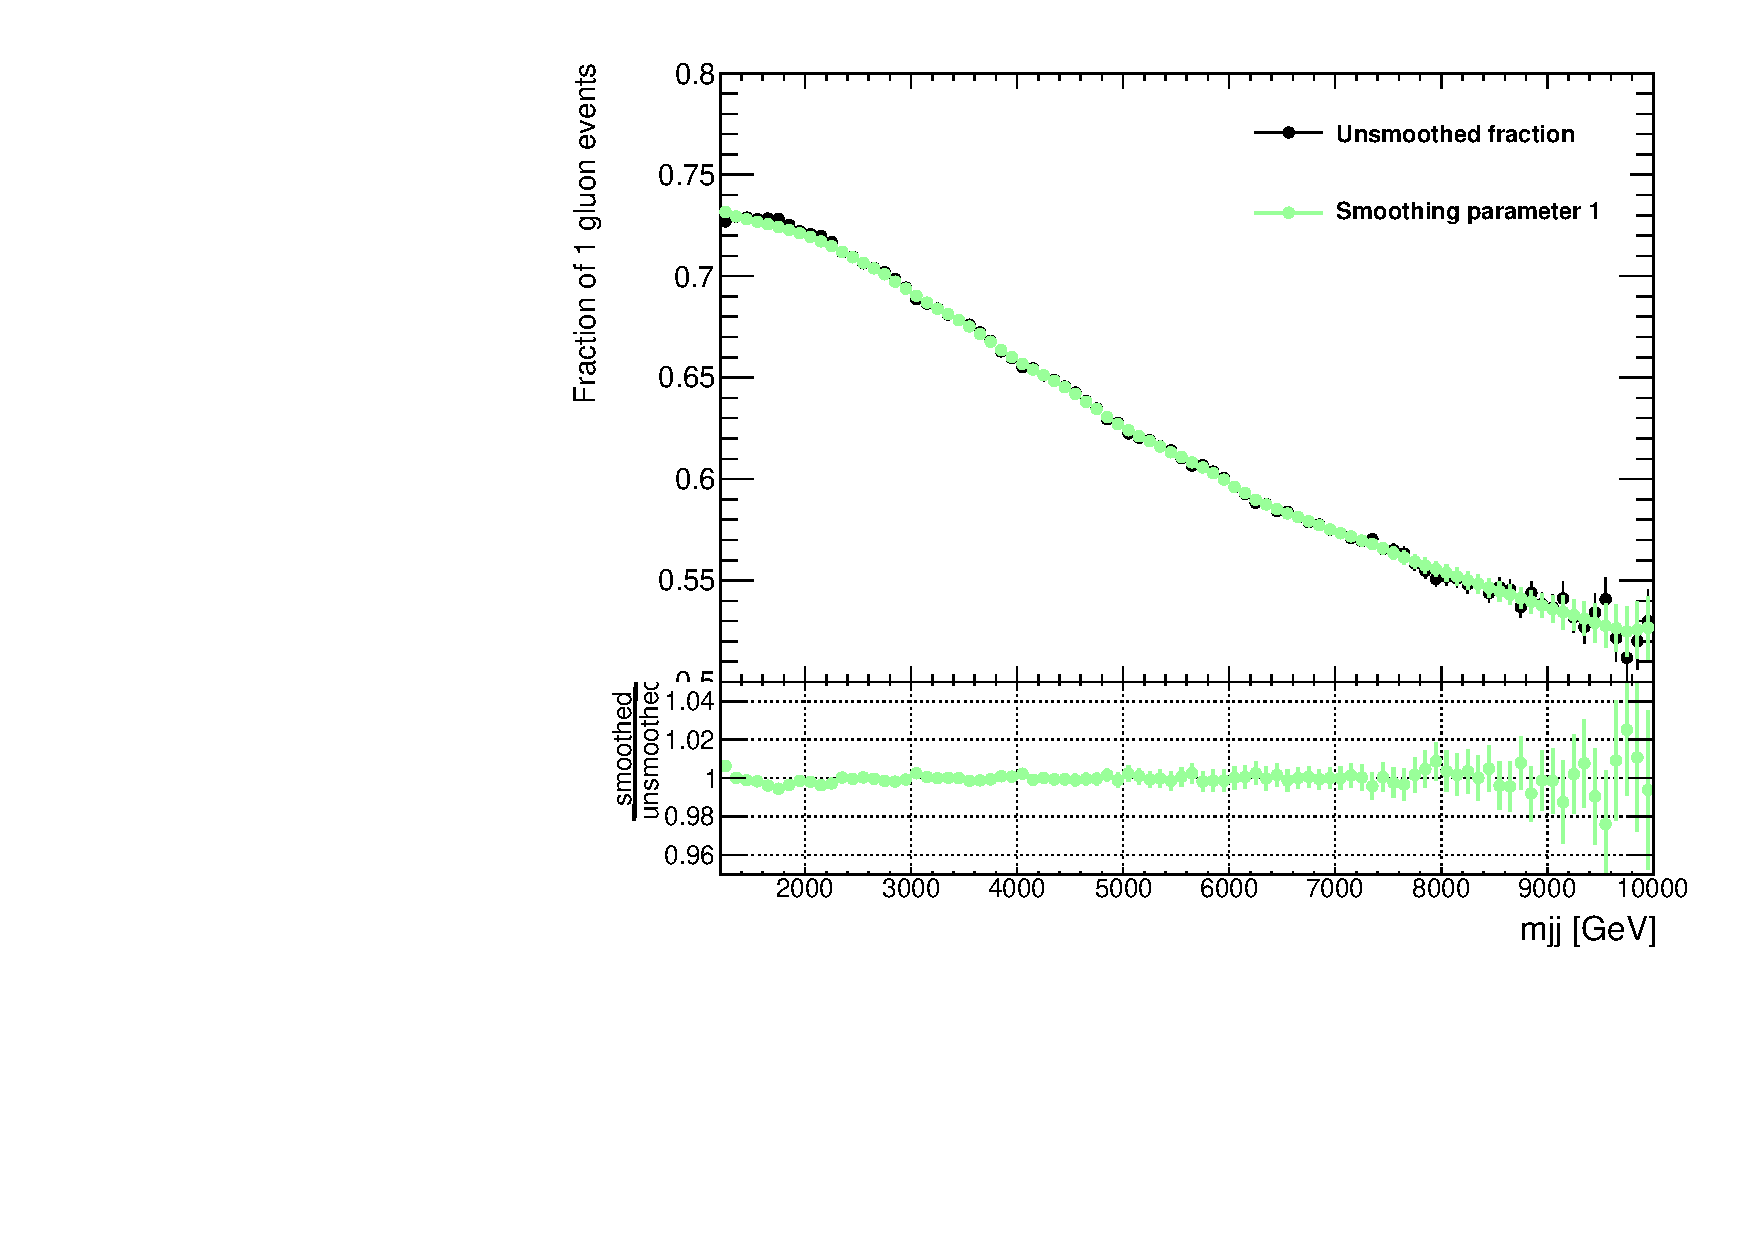
\includegraphics[width=0.48\columnwidth]{fig/pseudodata/Fraction_1gluon_Alpha10to0}}
%
%        \caption{Smoothed fraction of events passing 1 gluon tag selection using smoothing parameter of
%        (a) 1 (b) 7 (c) 8 and (d) 10.}
%        \label{fig:smoothFractions_1gtag}
%\end{figure}
%
%The pseudo-data generated for the 1 gluon tag category can be seen in Figure~\ref{fig:pseudodata_1gtag}.
%
% \begin{figure}[!htb]
%   \centering
%   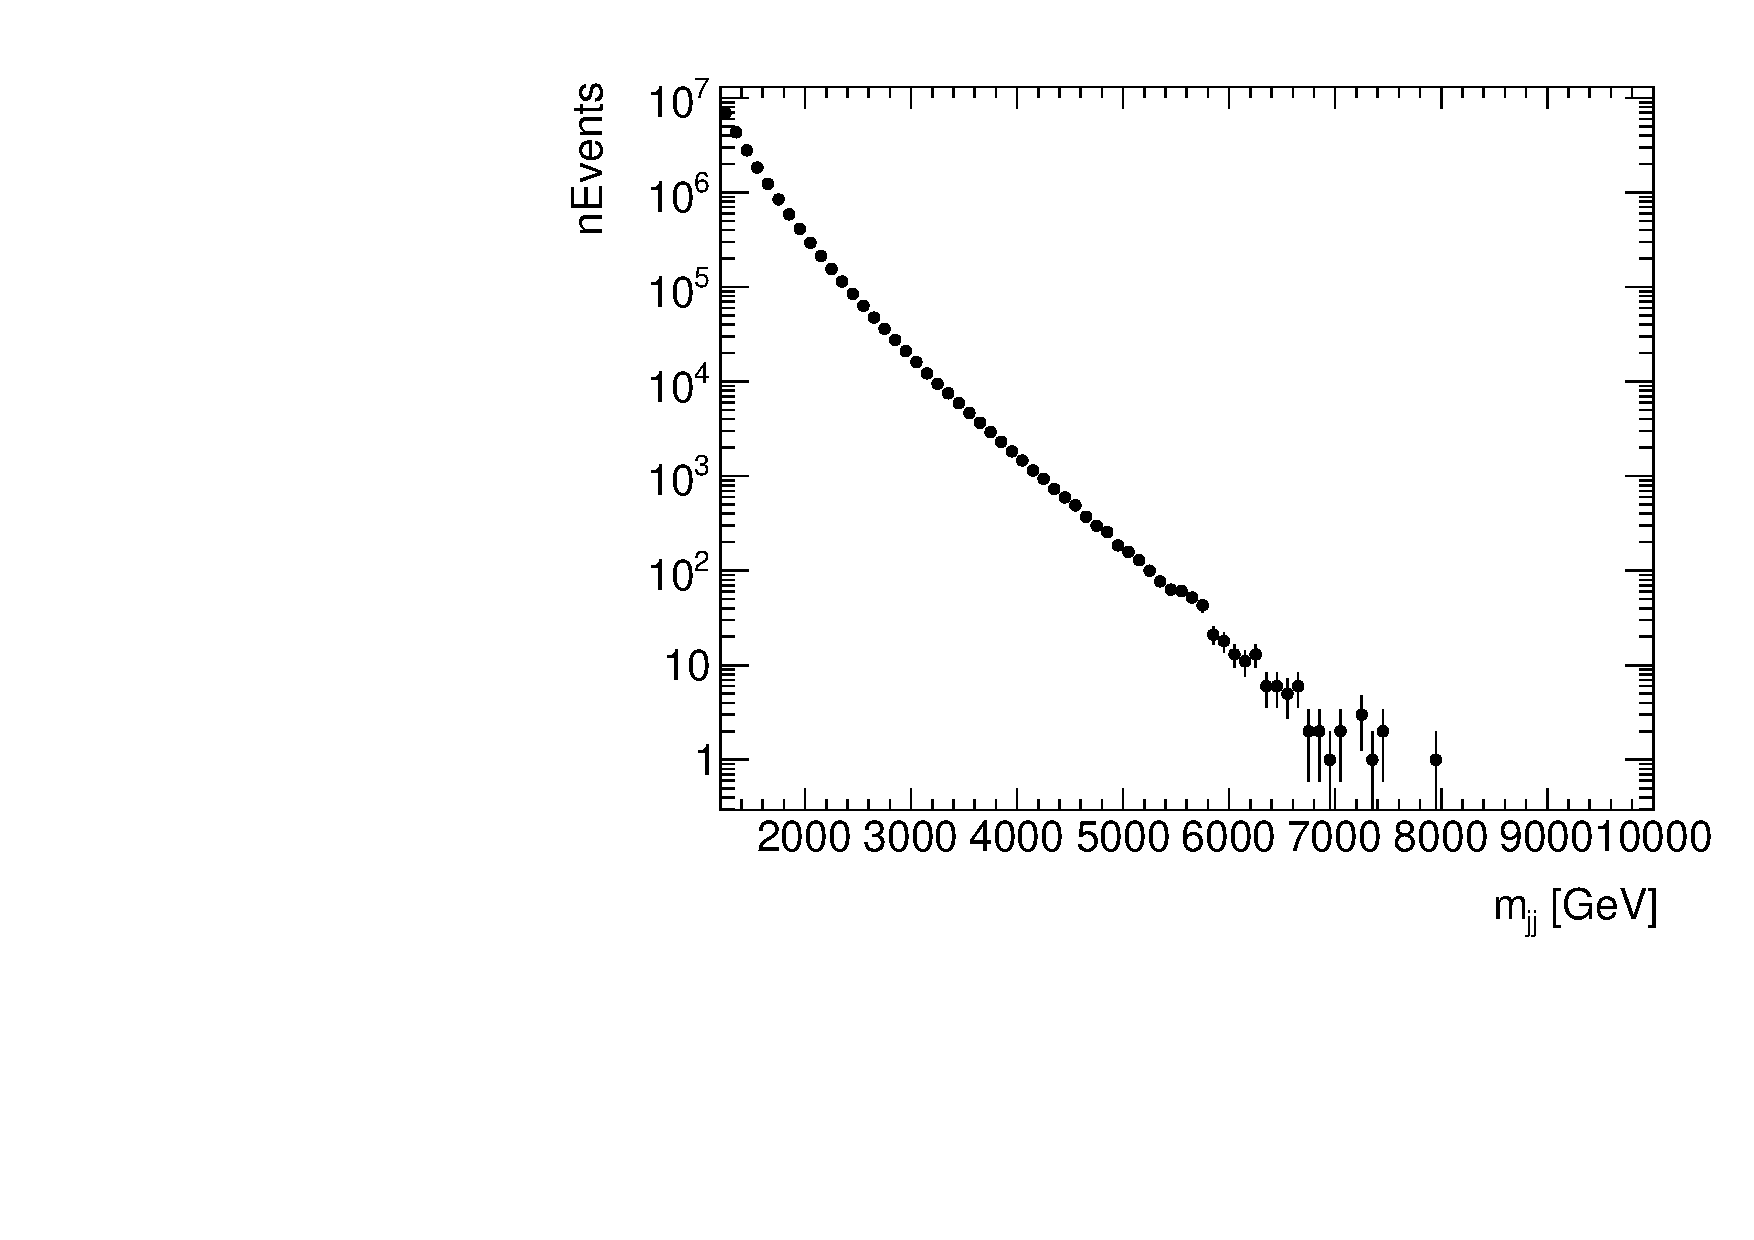
\includegraphics[width=0.45\textwidth]{fig/pseudodata/Pseudodata_1gluonTag.pdf}
%   \caption{Pseudodata for 1 gluon tag category.
%   \label{fig:pseudodata_1gtag}}
% \end{figure}
%
%The same procedure was followed to obtain the pseudo-data for the 2 gluon tag category using $|\ystar|<0.6$ and \mjj\ > 1100\,\GeV.
%Figure~\ref{fig:mjjFit_ystar0p6} shows the fitted untagged spectrum with 5-parameter global fit function using Minuit2 and figure~\ref{fig:fraction_2gtag_unsmooth} shows the fraction of events passing 2 gluon tag selection.
%Figure~\ref{fig:smoothFractions_2gtag} shows the smoothed fraction of events passing two gluon tag selection along with the ratios to the unsmoothed fractions. For the 2 gluon tag category, smoothing parameter 7 (Figure.~\ref{fig:smoothFractions_2gtag}(b)) was used.  The pseudo-data
%generated for the 2 gluon tag category can be seen in Figure~\ref{fig:pseudodata_2gtag}.
%
% \begin{figure}[!htb]
%   \centering
%   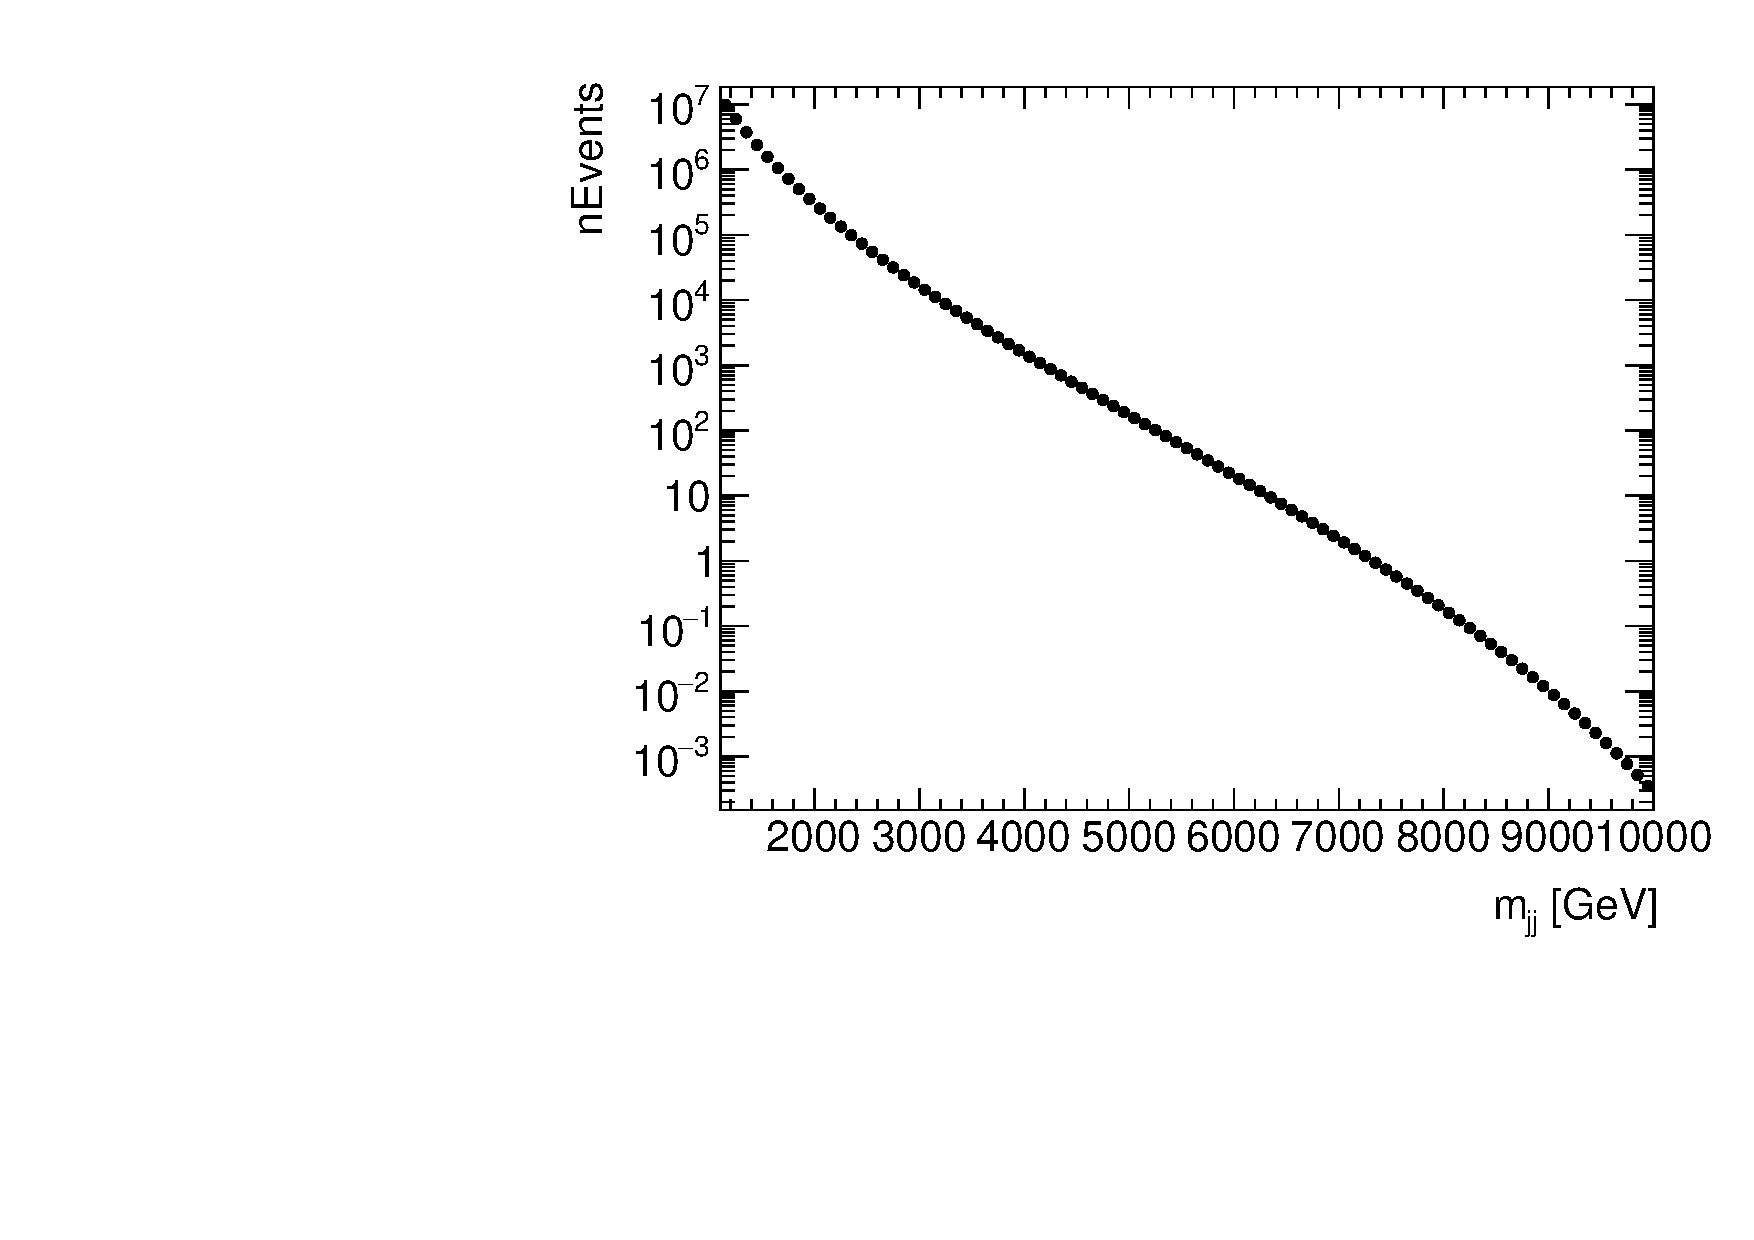
\includegraphics[width=0.45\textwidth]{fig/pseudodata/FittedMjj_UntaggedData_yStar0p6}
%   \caption{Untagged dijet spectrum with $|\ystar|<0.6$ using Full Run-2 data fitted with 5 parameter global fit.
%   \label{fig:mjjFit_ystar0p6}}
% \end{figure}
%
% \begin{figure}[!htb]
%   \centering
%   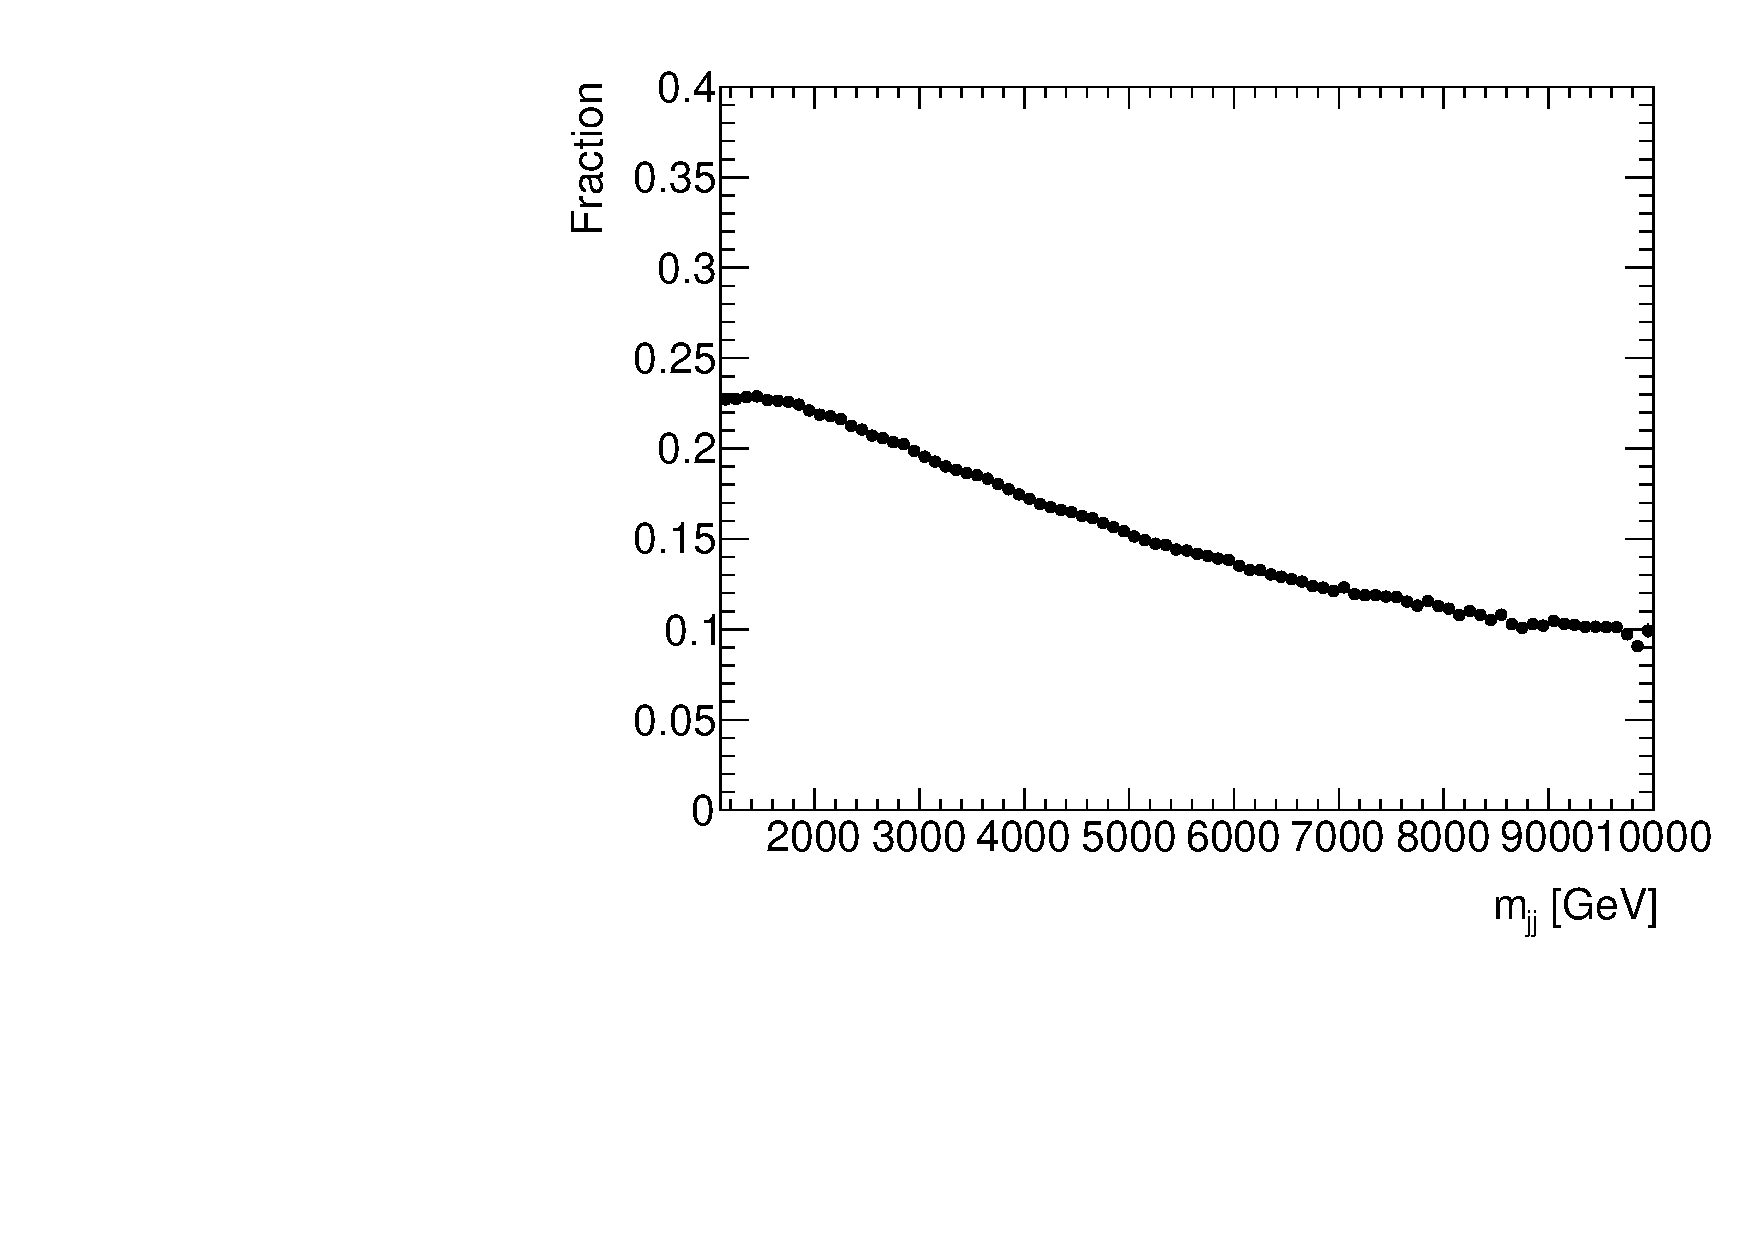
\includegraphics[width=0.45\textwidth]{fig/pseudodata/FractionUnsmooth_2gtag_yStar0p6}
%   \caption{Fraction of events passing 2 gluon tag selection.
%   \label{fig:fraction_2gtag_unsmooth}}
% \end{figure}
%
%\begin{figure}[htbp]
%        \centering
%        \subfloat[Smoothing parameter 4]{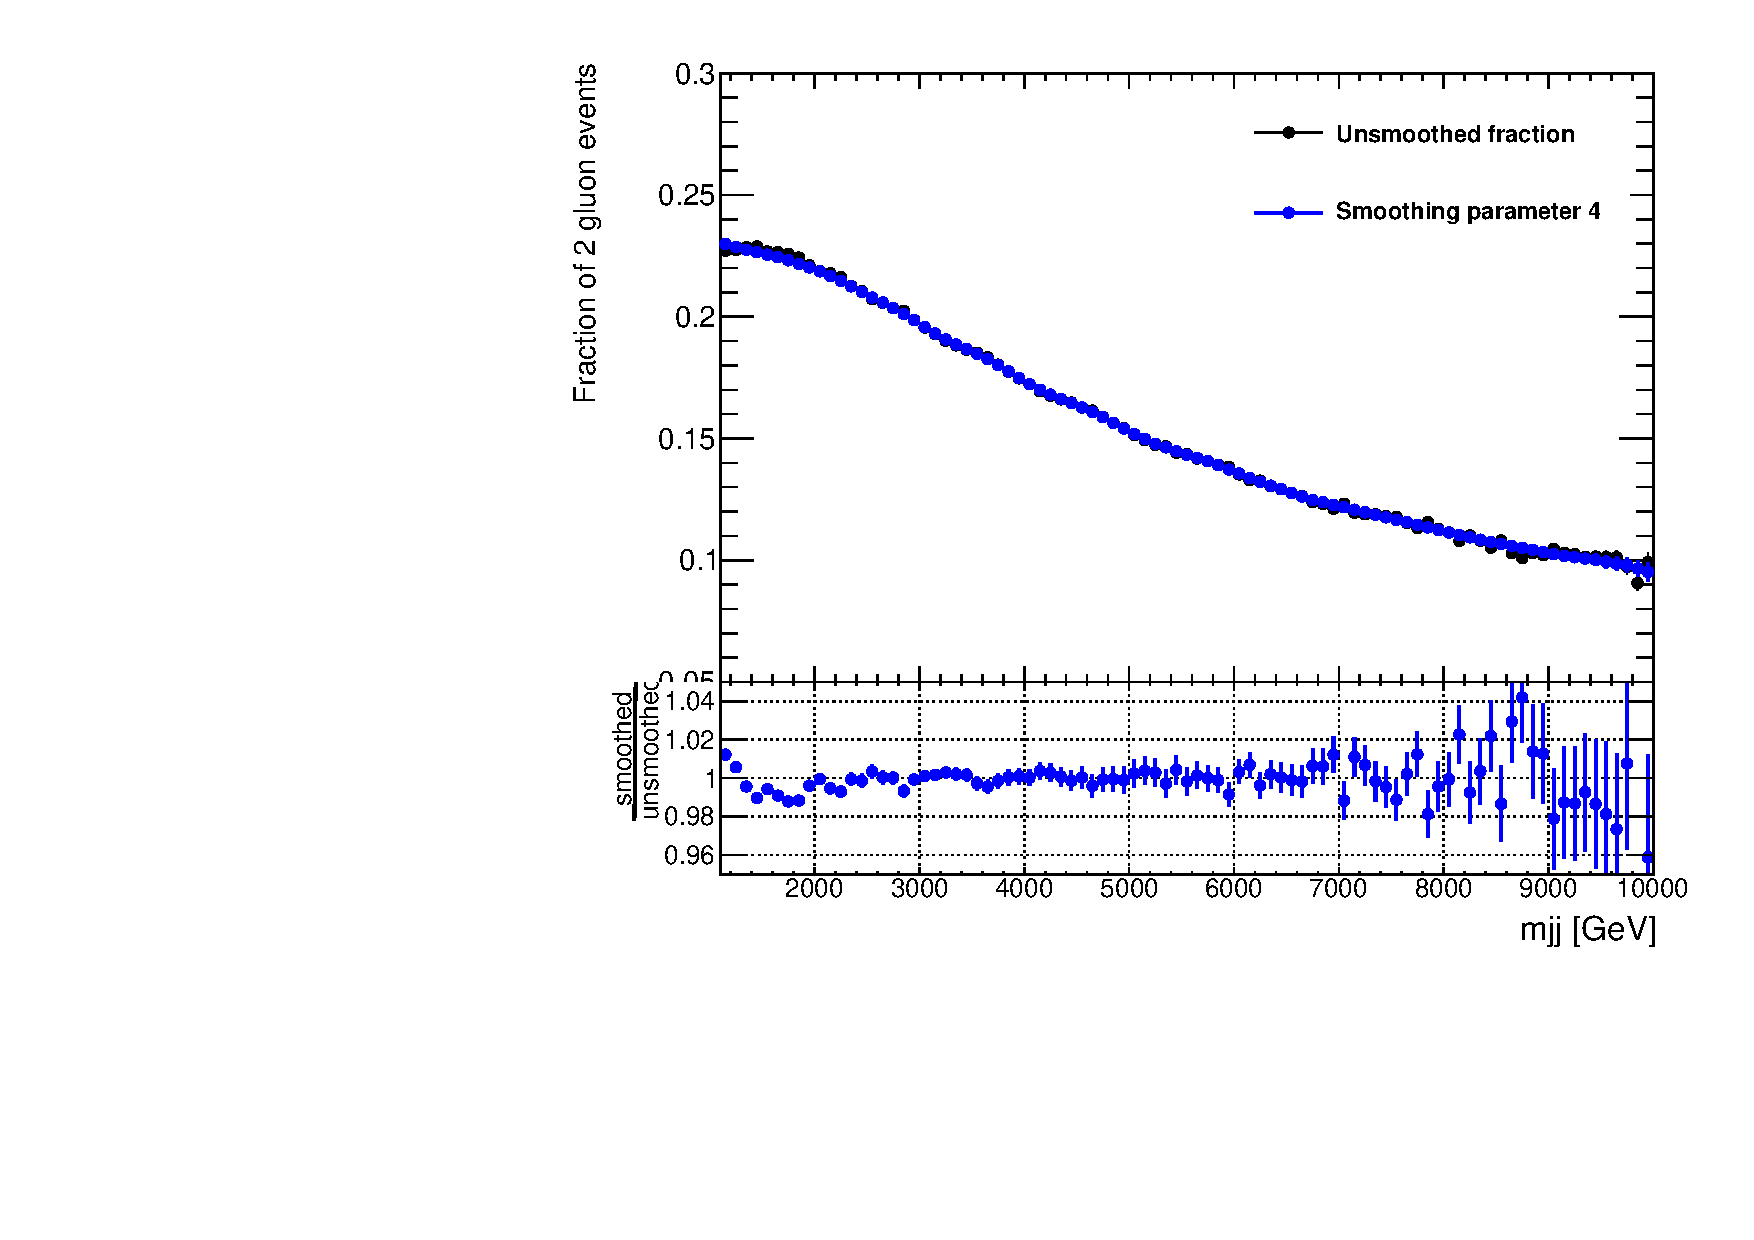
\includegraphics[width=0.48\columnwidth]{fig/pseudodata/Fraction_2gluon_Alpha4to0}}
%        \subfloat[Smoothing parameter 6]{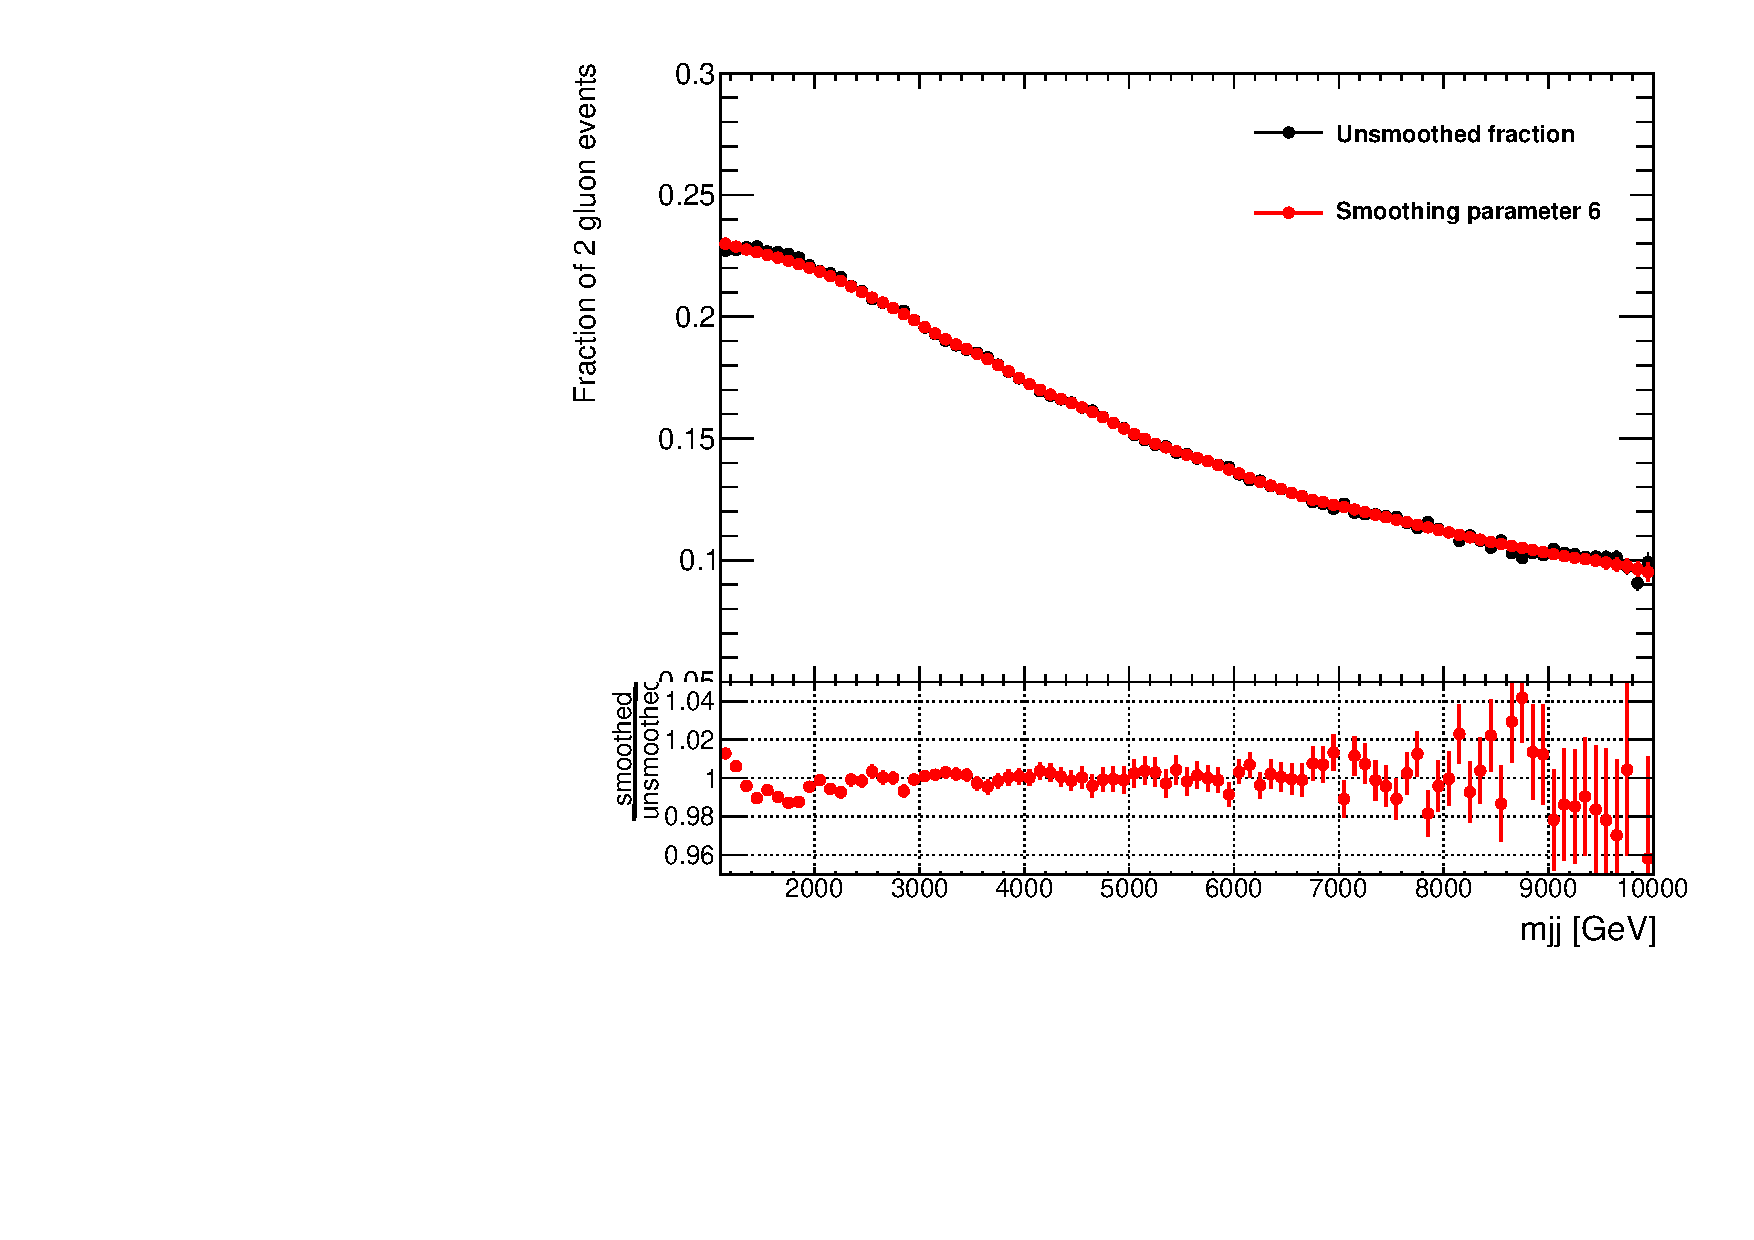
\includegraphics[width=0.48\columnwidth]{fig/pseudodata/Fraction_2gluon_Alpha6to0}}
%        \\
%        \subfloat[Smoothing parameter 8]{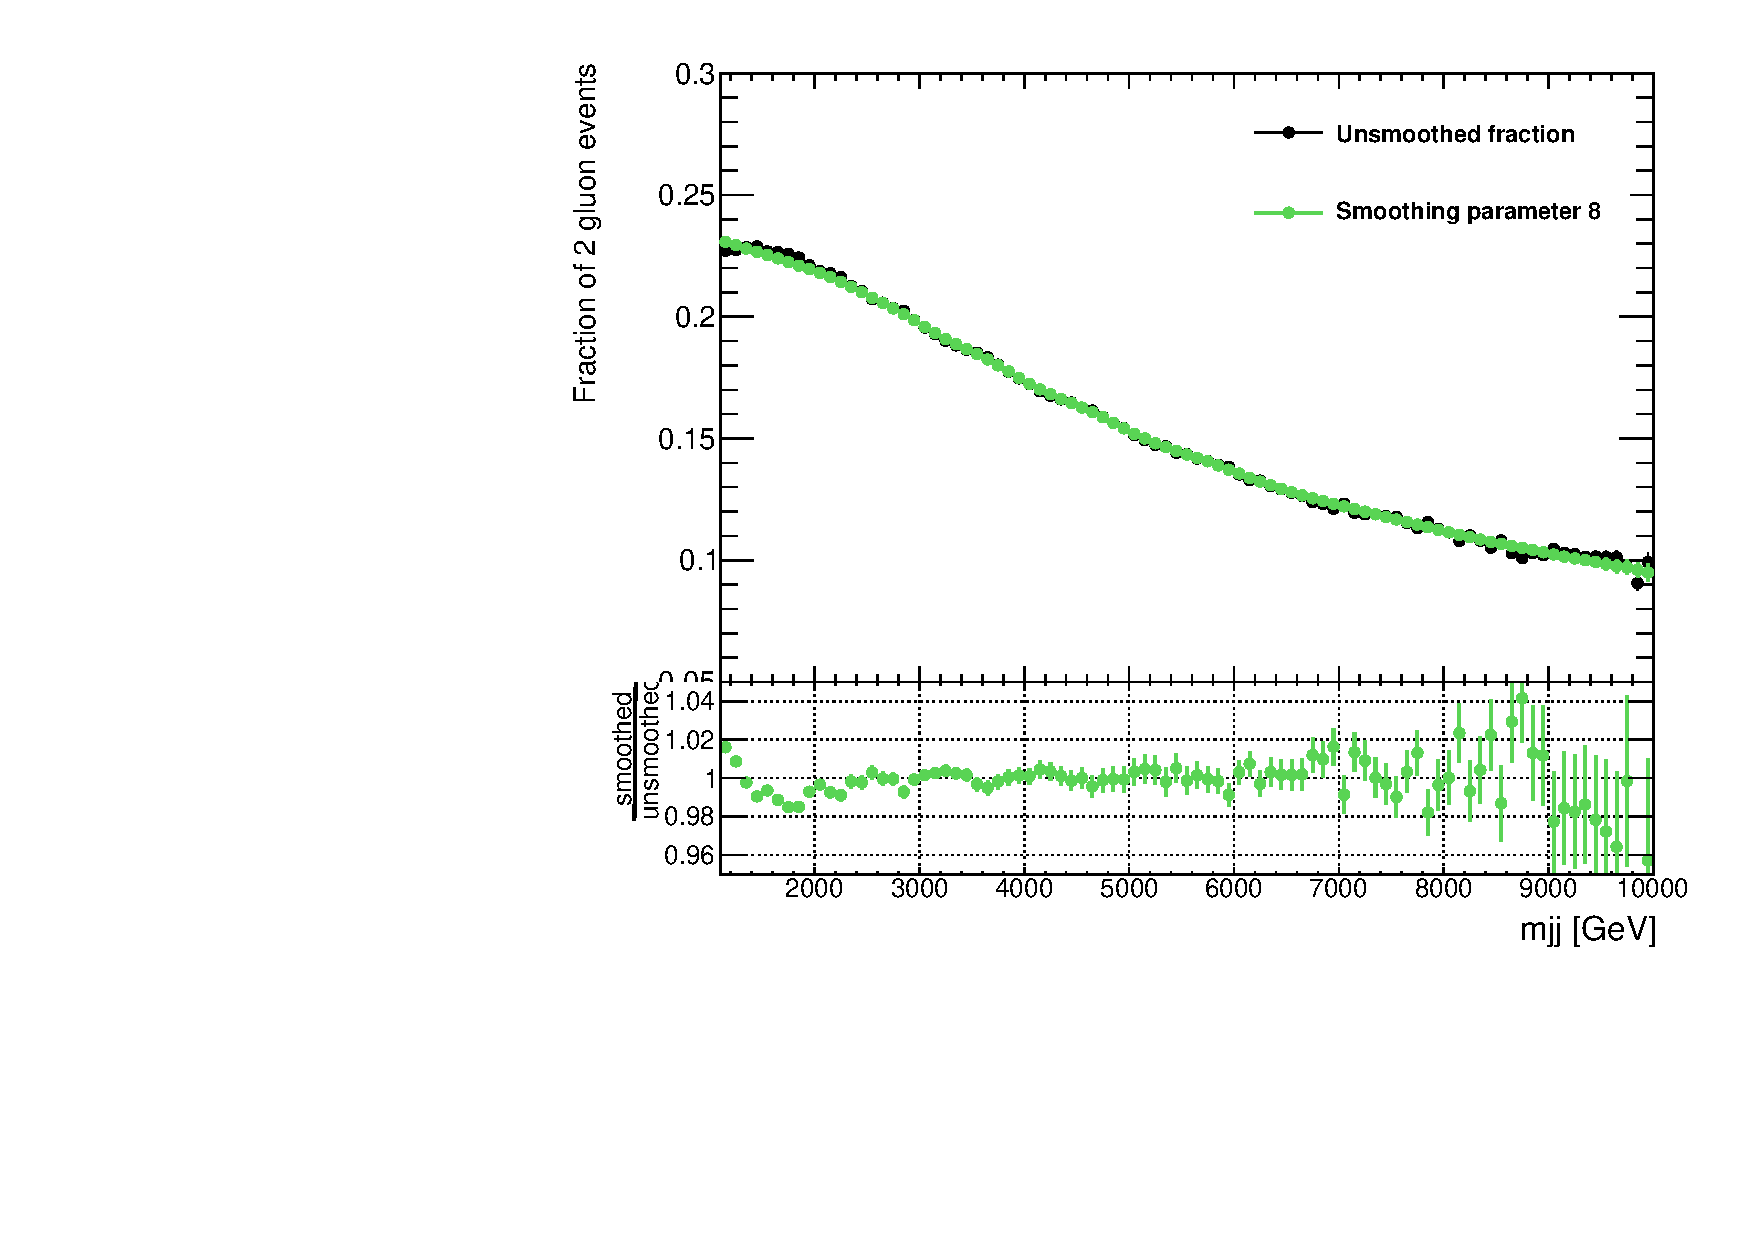
\includegraphics[width=0.48\columnwidth]{fig/pseudodata/Fraction_2gluon_Alpha8to0}}
%        \subfloat[Smoothing parameter 10]{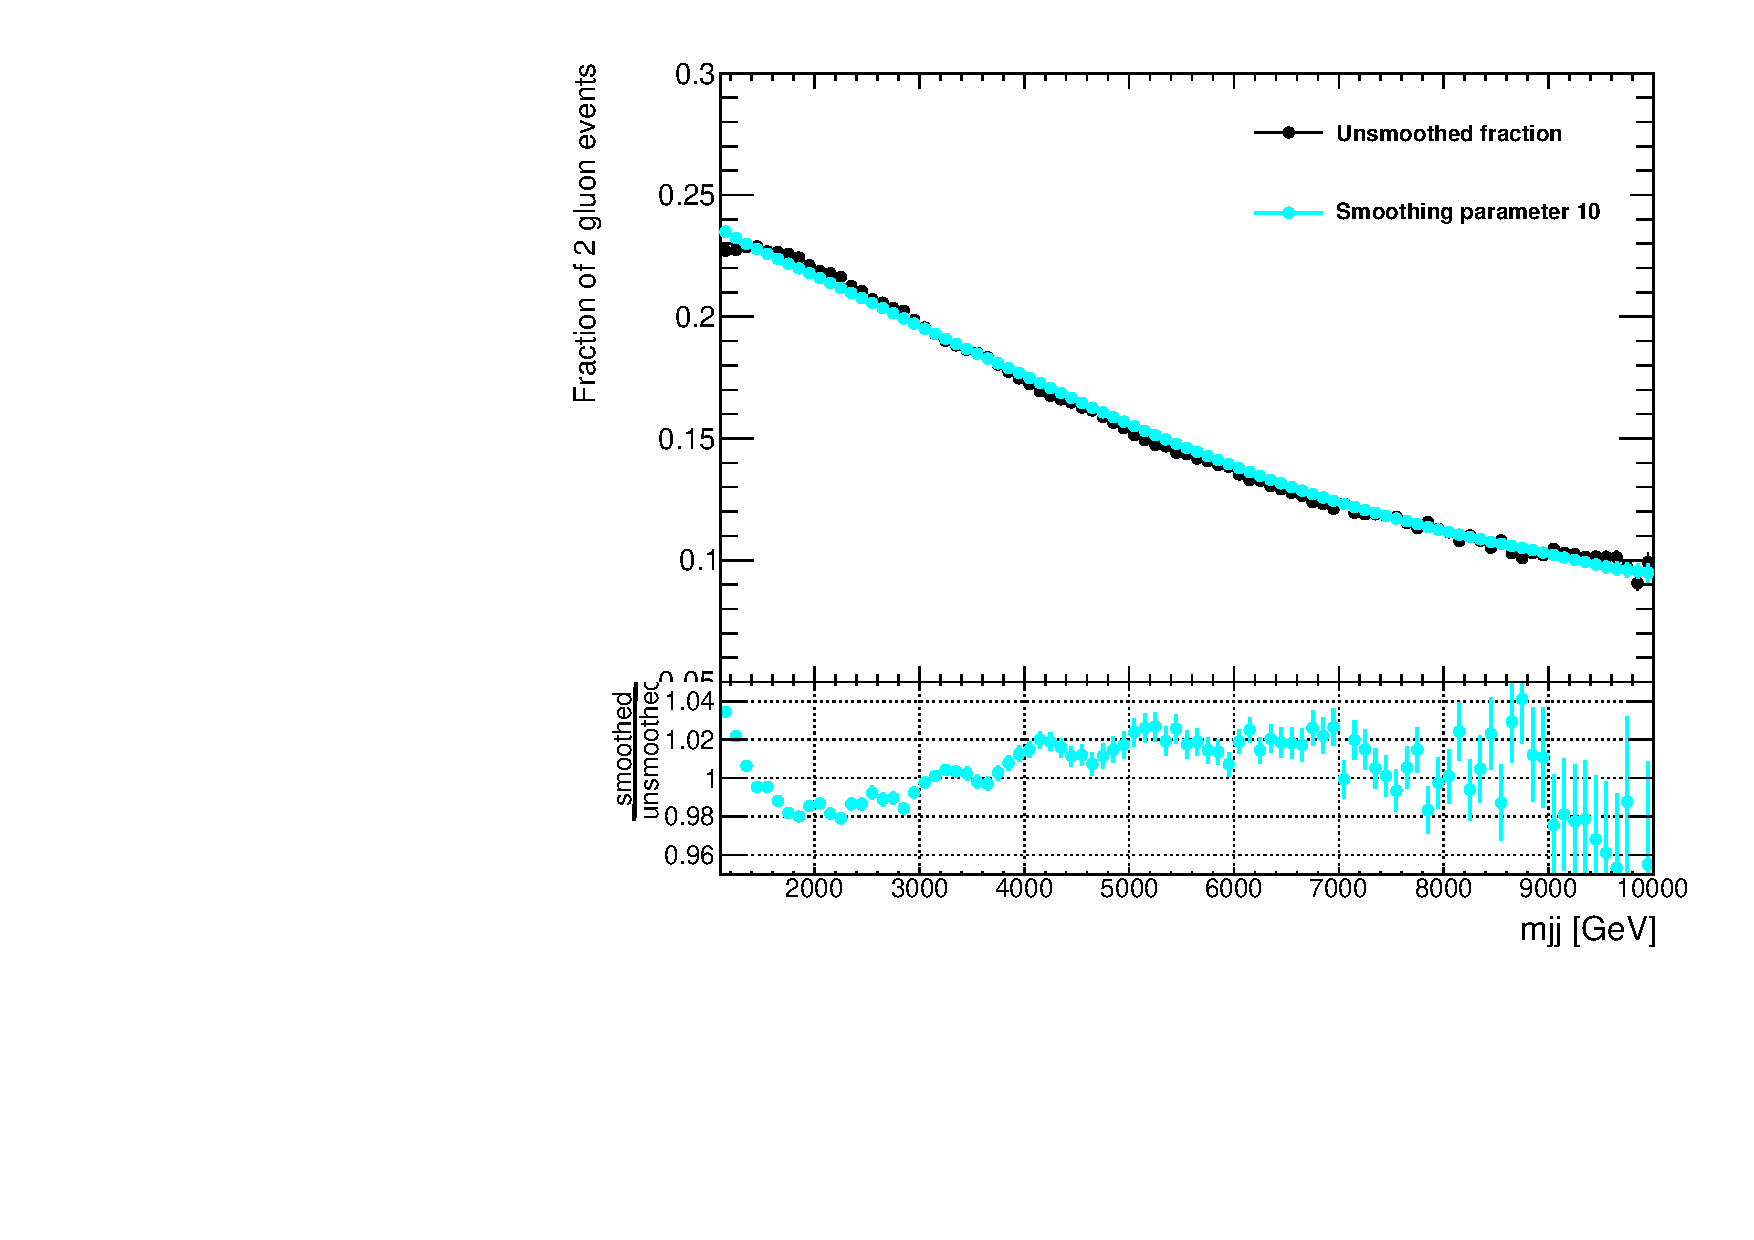
\includegraphics[width=0.48\columnwidth]{fig/pseudodata/Fraction_2gluon_Alpha10to0}}
%        \caption{Smoothed fraction of events passing 2 gluon tag selection using smoothing parameter of
%        (a) 4 (b) 6 (c) 8 and (d) 10.}
%        \label{fig:smoothFractions_2gtag}
%\end{figure}
%
% \begin{figure}[!htb]
%   \centering
%   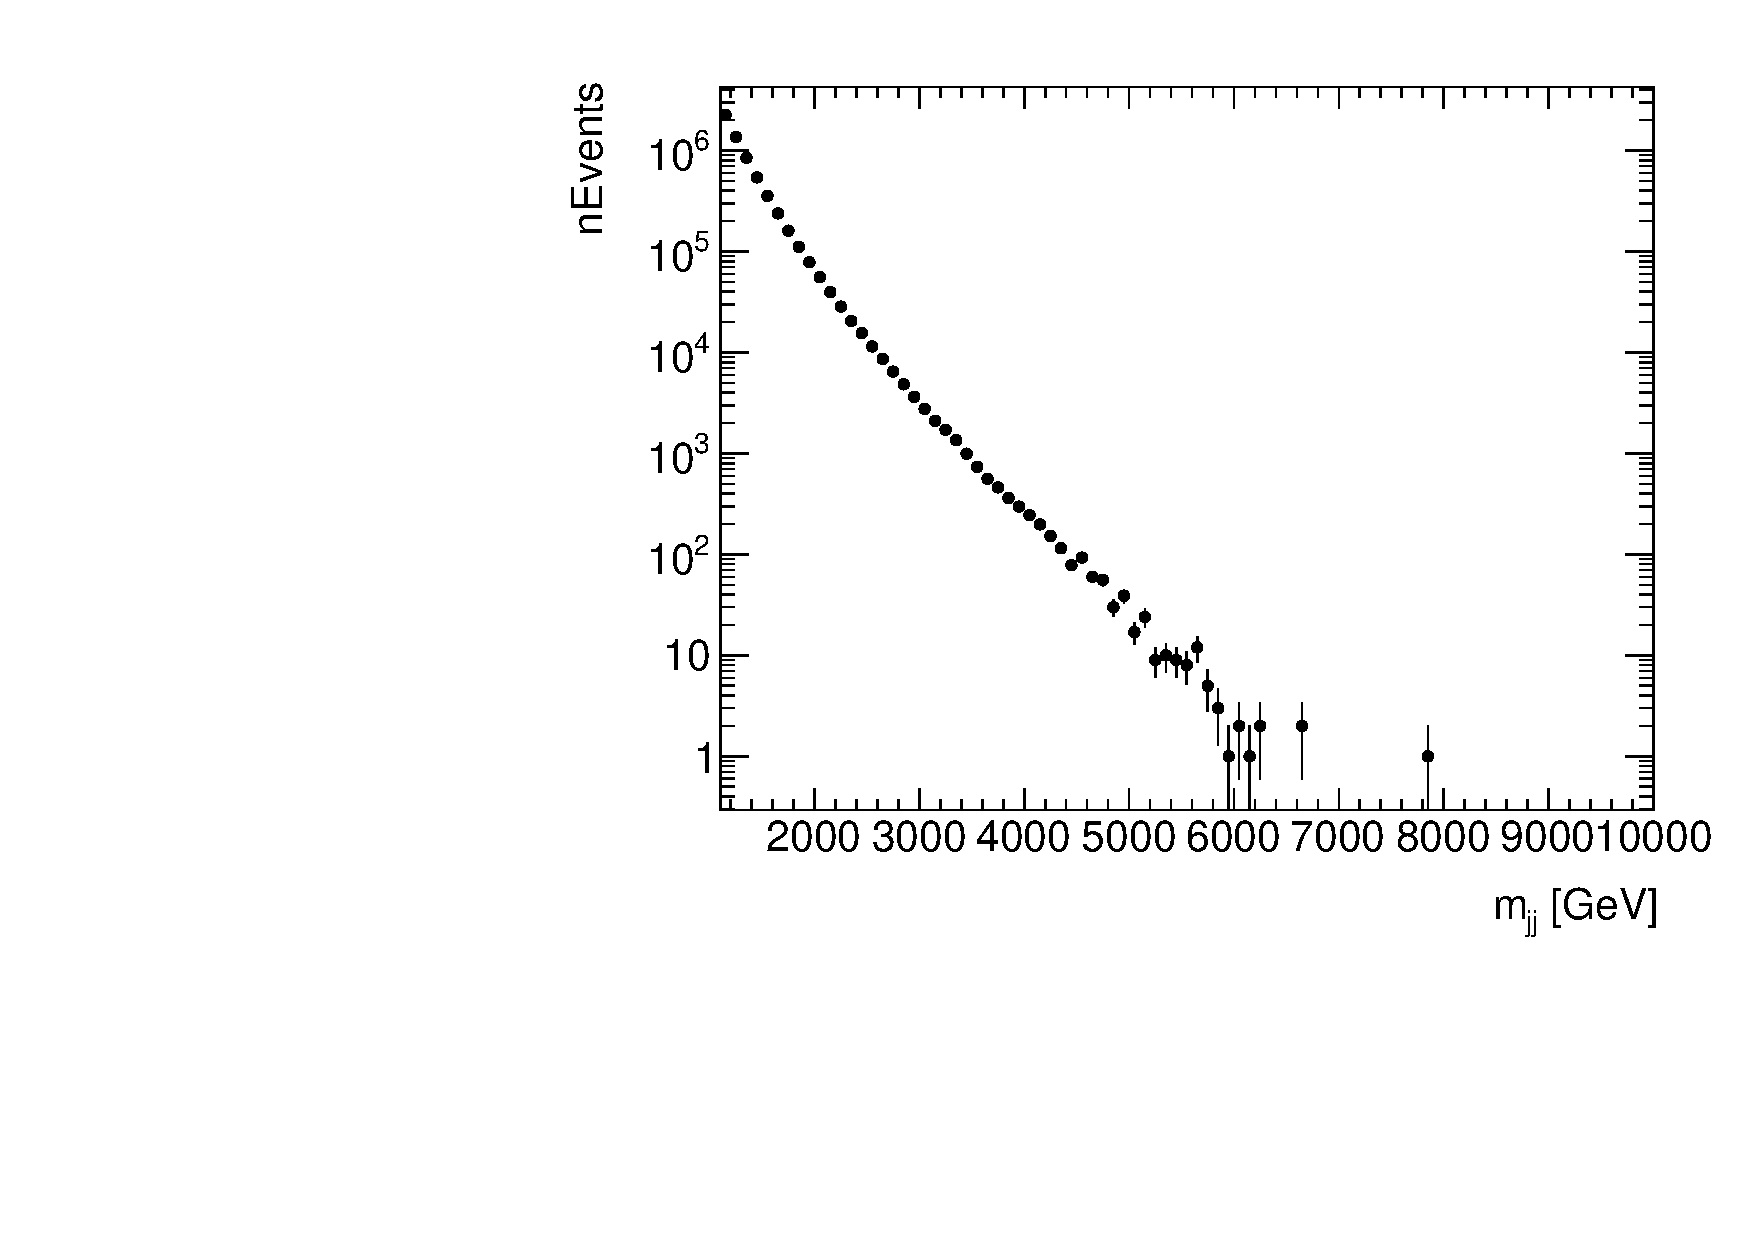
\includegraphics[width=0.45\textwidth]{fig/pseudodata/Pseudodata_2gluonTag.pdf}
%   \caption{Pseudodata for 2 gluon tag category.
%   \label{fig:pseudodata_2gtag}}
% \end{figure}
%
%\FloatBarrier

\subsubsection{Spurious signal tests}

The spurious signal test is designed to estimate the difference between the signal yields from the fit and the expected signal yields that given by fitting a known template signal model on a smooth background distribution. Such difference is considered as fit bias and defined as $S_\mathrm{spur}$:

\begin{equation}
 S_\mathrm{spur} = S_\mathrm{fit} - S_\mathrm{template}
\end{equation}

It is crucial to verify the stability of the fit when applied to a background-only distribution. In this context, no signal is intentionally introduced into the yields, ensuring that the extracted number of signal events remains zero. In the spurious signal test, $S_\mathrm{spur}$ is determined by fitting a model comprising both signal and background components onto a background-only template. The corresponding uncertainty from the fit is denoted as $\sigma_\mathrm{fit}$. Both the spurious signal $S_\mathrm{spur}$ and its associated uncertainty $\sigma_\mathrm{fit}$ are expected to be consistent with zero.

The estimation of the spurious signal is consequently conducted through these pseudo-experiments. The mean value across all experiments is calculated, and a total of 100 pseudo-experiments have been employed. For each individual signal hypothesis, the assessment of spurious signals is conducted at various mass points. The outcomes of the model-independent tests for Gaussian signals, considering different masses and widths, are consolidated in Table~\ref{tab:Sspur_Gauss_1gtag} for the 1 gluon-tagged category and in Table~\ref{tab:Sspur_Gauss_2gtag} for the 2 gluon-tagged category. %Correspondingly, the findings for string signals characterized by different string scales are presented in Table~\ref{tab:Sspur_String_1gtag}.

\begin{table}[ht]
\begin{center}
\renewcommand{\arraystretch}{1.4}
\begin{tabular}{ccl@{\,}@{$\pm$}@{\,}lc}
\toprule
Mass & Width & \multicolumn{2}{c}{Median $\pm$ Rms} & Ratio \\
 TeV & percentage [\%] & \multicolumn{2}{c}{$S_\mathrm{spurious}$ $\pm$ Uncertainty} & $S_\mathrm{spurious}$/Uncertainty \\
\midrule
2  & 5  & \numRP{0.19    }{2} & \numRP{802.85 }{2}    & \numRP{2.36E-04}{2}\\
2  & 10 & \numRP{3.35    }{2} & \numRP{1313.79}{2}    & \numRP{2.55E-03}{2}\\
2  & 15 & \numRP{154.92  }{2} & \numRP{1666.6 }{2}    & \numRP{0.093   }{2}\\
3  & 5  & \numRP{1.76    }{2} & \numRP{249.13 }{2}    & \numRP{7.06E-03}{2}\\
3  & 10 & \numRP{82.55   }{2} & \numRP{520.85 }{2}    & \numRP{0.158   }{2}\\
3  & 15 & \numRP{344.74  }{2} & \numRP{803.85 }{2}    & \numRP{0.429   }{2}\\
4  & 5  & \numRP{48.42   }{2} & \numRP{112.34 }{2}    & \numRP{0.431   }{2}\\
4  & 10 & \numRP{115.89  }{2} & \numRP{200.83 }{2}    & \numRP{0.577   }{2}\\
4  & 15 & \numRP{2.02    }{2} & \numRP{242.15 }{2}    & \numRP{8.34E-03}{2}\\
5  & 5  & \numRP{0.021   }{2} & \numRP{31.77  }{2}    & \numRP{6.61E-04}{2}\\
5  & 10 & \numRP{0.012   }{2} & \numRP{31.96  }{2}    & \numRP{3.75E-04}{2}\\
5  & 15 & \numRP{0.006   }{2} & \numRP{18.98  }{2}    & \numRP{3.16E-04}{2}\\
6  & 5  & \numRP{7.82E-04}{2} & \numRP{5.54   }{2}    & \numRP{1.41E-04}{2}\\
6  & 10 & \numRP{2.84E-04}{2} & \numRP{5.93   }{2}    & \numRP{4.79E-05}{2}\\
6  & 15 & \numRP{3.62E-04}{2} & \numRP{5.79   }{2}    & \numRP{6.25E-05}{2}\\
7  & 5  & \numRP{8.65E-04}{2} & \numRP{2.66   }{2}    & \numRP{3.25E-04}{2}\\
7  & 10 & \numRP{1.6E-04 }{2} & \numRP{2.59   }{2}    & \numRP{6.18E-05}{2}\\
7  & 15 & \numRP{8.34E-05}{2} & \numRP{2.71   }{2}    & \numRP{3.08E-05}{2}\\
\bottomrule
\end{tabular}
\end{center}
\caption{Spurious Signal tests using Gaussian signals for 1 gluon tagged category.}
\label{tab:Sspur_Gauss_1gtag}
\end{table}%

\begin{table}[ht]
\begin{center}
\renewcommand{\arraystretch}{1.4}
\begin{tabular}{ccl@{\,}@{$\pm$}@{\,}lc}
\toprule
Mass & Width & \multicolumn{2}{c}{Median $\pm$ Rms} & Ratio \\
 TeV & percentage [\%] & \multicolumn{2}{c}{$S_\mathrm{spurious}$ $\pm$ Uncertainty} & $S_\mathrm{spurious}$/Uncertainty \\
\midrule
2  & 5  & \numRP{179.84  }{2} & \numRP{635.08     }{2}    &  \numRP{0.283      }{2} \\
2  & 10 & \numRP{757.07  }{2} & \numRP{1265.99    }{2}    &  \numRP{0.598      }{2} \\
2  & 15 & \numRP{1666.24 }{2} & \numRP{2126.08    }{2}    &  \numRP{0.784      }{2} \\
3  & 5  & \numRP{1.83E-03}{2} & \numRP{85.31      }{2}    &  \numRP{2.14E-05   }{2} \\
3  & 10 & \numRP{0.27    }{2} & \numRP{125.63     }{2}    &  \numRP{2.15E-03   }{2} \\
3  & 15 & \numRP{0.021   }{2} & \numRP{113.74     }{2}    &  \numRP{1.85E-04   }{2} \\
4  & 5  & \numRP{1.91E-03}{2} & \numRP{25.6       }{2}    &  \numRP{7.46E-05   }{2} \\
4  & 10 & \numRP{3.55E-03}{2} & \numRP{38.68      }{2}    &  \numRP{9.18E-05   }{2} \\
4  & 15 & \numRP{1.50E-03}{2} & \numRP{27.01      }{2}    &  \numRP{5.55E-05   }{2} \\
5  & 5  & \numRP{2.72E-04}{2} & \numRP{7.13       }{2}    &  \numRP{3.81E-05   }{2} \\
5  & 10 & \numRP{9.99E-05}{2} & \numRP{5.57       }{2}    &  \numRP{1.79E-05   }{2} \\
5  & 15 & \numRP{2.1E-04 }{2} & \numRP{4.72       }{2}    &  \numRP{4.45E-05   }{2} \\
6  & 5  & \numRP{1.37E-04}{2} & \numRP{1.92       }{2}    &  \numRP{7.14E-05   }{2} \\
6  & 10 & \numRP{1.47E-04}{2} & \numRP{3.25       }{2}    &  \numRP{4.52E-05   }{2} \\
6  & 15 & \numRP{6.49E-05}{2} & \numRP{2.59       }{2}    &  \numRP{2.51E-05   }{2} \\
7  & 5  & \numRP{1.88E-04}{2} & \numRP{1.19       }{2}    &  \numRP{1.58E-04   }{2} \\
7  & 10 & \numRP{1.17E-04}{2} & \numRP{1.17       }{2}    &  \numRP{1.0E-04    }{2} \\
7  & 15 & \numRP{7.83E-05}{2} & \numRP{1.20       }{2}    &  \numRP{6.53E-05   }{2} \\
\bottomrule
\end{tabular}
\end{center}
\caption{Spurious Signal tests using Gaussian signals for 2 gluon tagged category.}
\label{tab:Sspur_Gauss_2gtag}
\end{table}%

%
%\begin{table}[ht]
%\begin{center}
%\renewcommand{\arraystretch}{1.4}
%\begin{tabular}{cl@{\,}@{$\pm$}@{\,}lc}
%\toprule
%String scale & \multicolumn{2}{c}{Median $\pm$ Rms} & Ratio \\
% TeV  & \multicolumn{2}{c}{$S_\mathrm{spurious}$ $\pm$ Uncertainty} & $S_\mathrm{spurious}$/Uncertainty \\
%\midrule
%7    & \numRP{4.12E-04}{2} & \numRP{5.83}{2} & \numRP{7.07E-05}{2} \\
%7.5  & \numRP{1.6E-04 }{2} & \numRP{3.72}{2} & \numRP{2.84E-05}{2} \\
%8    & \numRP{6.77E-05}{2} & \numRP{2.11}{2} & \numRP{3.21E-05}{2} \\
%8.5  & \numRP{3.83E-05}{2} & \numRP{1.84}{2} & \numRP{2.08E-05}{2} \\
%9    & \numRP{3.87E-05}{2} & \numRP{1.93}{2} & \numRP{2.01E-05}{2} \\
%\bottomrule
%\end{tabular}
%\end{center}
%\caption{Spurious Signal tests using String signals.}
%\label{tab:Sspur_String_1gtag}
%\end{table}%

Following the recommendations of the Statistical PUB Note~\cite{ATL-PHYS-PUB-2020-028}
, the spurious signal is required to be
\begin{equation}
 S_\mathrm{spur} < (20\% - 50\%)\sigma_\mathrm{fit}
\end{equation}

The idea criteria is when the spurious signal satisfy: $S_\mathrm{spur}$ < 30\% $\sigma_\mathrm{fit}$, but can be loosen up to 50\% $\sigma_\mathrm{fit}$. Most of the tested mass points and widths satisfy the spurious signal criteria. 

\FloatBarrier

\subsubsection{Fit stability tests}
The fit stability tests are employed to assess the behaviour of the background fit function under different scenarios: when applied to the background-only template and the signal + background template. A comparison is made between the fit results obtained from these two templates. Ideally, the background fit function should yield consistent outcomes in both cases. The results of these fit stability tests are presented in Table~\ref{tab:FitStab_Gauss_1gtag} through Table~\ref{tab:FitStab_Gauss_2gtag}, encompassing various signal strengths and mass points.

Notably, the background estimation derived from the signal + background fit ($B_1$) aligns with the background estimation obtained from the background-only fit ($B_2$), indicating good agreement between the two approaches.

\begin{table}[ht]
\begin{center}
\renewcommand{\arraystretch}{1.4}
\resizebox{0.95\textwidth}{!}{
\begin{tabular}{cccl@{\,}@{$\pm$}@{\,}ll@{\,}@{$\pm$}@{\,}c}
\toprule
Mass & Width & Signal  & \multicolumn{2}{c}{$B_1$ from S+B fit} & \multicolumn{2}{c}{$B_2$ from B-only fit} \\
(TeV)  & (percentage) & Strength  & \multicolumn{2}{c}{Mean $\pm$ Rms} & \multicolumn{2}{c}{Mean $\pm$ Rms}  \\
\midrule
2  & 5  & 1 & \numRP{20062716.45}{2} & \numRP{4370.57}{2} & \numRP{20064025.61}{2} & \numRP{4003.07}{2} \\
2  & 5  & 3 & \numRP{20063730.27}{2} & \numRP{4882.09}{2} & \numRP{20067248.18}{2} & \numRP{4003.14}{2}  \\
2  & 5  & 5 & \numRP{20062961.53}{2} & \numRP{4521.62}{2} & \numRP{20070470.90}{2} & \numRP{4003.36}{2}  \\
5  & 5  & 1 & \numRP{20062414.49}{2} & \numRP{4005.80}{2} & \numRP{20062458.64}{2} & \numRP{4003.05}{2} \\
5  & 5  & 3 & \numRP{20062420.85}{2} & \numRP{4002.94}{2} & \numRP{20062547.11}{2} & \numRP{4003.09}{2}  \\
5  & 5  & 5 & \numRP{20062420.96}{2} & \numRP{4002.82}{2} & \numRP{20062635.82}{2} & \numRP{4003.25}{2} \\
5  & 10 & 1 & \numRP{20062435.18}{2} & \numRP{4010.37}{2} & \numRP{20062483.50}{2} & \numRP{4002.87}{2}  \\
5  & 10 & 3 & \numRP{20062448.75}{2} & \numRP{4007.22}{2} & \numRP{20062622.26}{2} & \numRP{4002.95}{2} \\
5  & 10 & 5 & \numRP{20061413.12}{2} & \numRP{3682.05}{2} & \numRP{20062761.08}{2} & \numRP{4003.12}{2} \\
7  & 5  & 1 & \numRP{20062420.38}{2} & \numRP{4002.68}{2} & \numRP{20062420.29}{2} & \numRP{4002.98}{2} \\
7  & 5  & 3 & \numRP{20062422.56}{2} & \numRP{4002.86}{2} & \numRP{20062432.08}{2} & \numRP{4003.08}{2} \\
7  & 5  & 5 & \numRP{20062422.86}{2} & \numRP{4002.98}{2} & \numRP{20062444.09}{2} & \numRP{4003.20}{2} \\
\bottomrule
\end{tabular}}
\end{center}
\caption{Fit Stability tests using Gaussian signals for 1 gluon tagged category.}
\label{tab:FitStab_Gauss_1gtag}
\end{table}%

\begin{table}[ht]
\begin{center}
\renewcommand{\arraystretch}{1.4}
\resizebox{0.95\textwidth}{!}{
\begin{tabular}{cccl@{\,}@{$\pm$}@{\,}ll@{\,}@{$\pm$}@{\,}c}
\toprule
Mass & Width & Signal  & \multicolumn{2}{c}{$B_1$ from S+B fit} & \multicolumn{2}{c}{$B_2$ from B-only fit}  \\
(TeV)  & (percentage) & Strength  & \multicolumn{2}{c}{Mean $\pm$ Rms} & \multicolumn{2}{c}{Mean $\pm$ Rms}  \\
\midrule
2  & 5  & 1 & \numRP{3901512.92}{2} & \numRP{2163.27}{2} & \numRP{3902240.71}{2} & \numRP{2048.04}{2} \\
2  & 5  & 3 & \numRP{3901530.76}{2} & \numRP{2166.98}{2} & \numRP{3903253.55}{2} & \numRP{2047.37}{2}  \\
2  & 5  & 5 & \numRP{3901621.90}{2} & \numRP{2291.01}{2} & \numRP{3905032.95}{2} & \numRP{2050.68}{2}  \\
5  & 5  & 1 & \numRP{3901529.75}{2} & \numRP{2049.31}{2} & \numRP{3901559.92}{2} & \numRP{2046.18}{2} \\
5  & 5  & 3 & \numRP{3901528.52}{2} & \numRP{2049.15}{2} & \numRP{3901589.41}{2} & \numRP{2044.93}{2}\\
5  & 5  & 5 & \numRP{3901533.99}{2} & \numRP{2047.48}{2} & \numRP{3901621.88}{2} & \numRP{3901586.68}{2} \\
5  & 10 & 1 & \numRP{3901536.86}{2} & \numRP{2047.40}{2} & \numRP{3901566.44}{2} & \numRP{2048.23}{2} \\
5  & 10 & 3 & \numRP{3901535.71}{2} & \numRP{2054.62}{2} & \numRP{3901616.49}{2} & \numRP{2050.26}{2}  \\
5  & 10 & 5 & \numRP{3901538.47}{2} & \numRP{2049.54}{2} & \numRP{3901670.56}{2} & \numRP{2047.94}{2}  \\
7  & 5  & 1 & \numRP{3901531.27}{2} & \numRP{2047.30}{2} & \numRP{3901538.45}{2} & \numRP{2049.16}{2}  \\
7  & 5  & 3 & \numRP{3901540.72}{2} & \numRP{2068.73}{2} & \numRP{3901542.75}{2} & \numRP{2048.46}{2} \\
7  & 5  & 5 & \numRP{3901533.13}{2} & \numRP{2052.64}{2} & \numRP{3901540.09}{2} & \numRP{2048.94}{2}  \\
\bottomrule
\end{tabular}}
\end{center}
\caption{Fit Stability tests using Gaussian signals for 2 gluon tagged category.}
\label{tab:FitStab_Gauss_2gtag}
\end{table}%

\FloatBarrier

%\subsubsection{Signal Injection Tests}
%On the condition that background only fit well, signal region where signals likely existed could affect the performance of background fit. As the dijet fit functions are motivated by the distribution of  \mjj from the QCD theory, where the distribution should be smooth and monotonically decreasing, the effect after injecting a signal with small width should be negligible on the fit.
%
%Therefore, it is important to further verify the fit stability by performing a signal injection test. The signal injection tests is carried out by fitting a signal + background template using a a signal + background model. Signal events with related width at each mass point are injected to the template for various signal strengths, which is then used for pseudo-experiments generation. In total 100 pseudo-experiments is used in this study.
%
%Gaussian signals are used in signal injection tests with different widths and mass points. Figure~\ref{fig:SigInj_1gtag} shows the 
%results of signal injection tests for the 1 gluon tag category and Figure~\ref{fig:SigInj_2gtag} 
%shows the results of signal injection tests for the 2 gluon tag category.
%The extracted number of signal events are consistent with the injected ones in most cases. There are some discrepancies and large error 
%bars for 2 TeV 15\% Gaussian signals due to some problems with fit convergence and are under investigation.
%
%\begin{figure}[htb]
%\centering
% %
%\subfloat[] {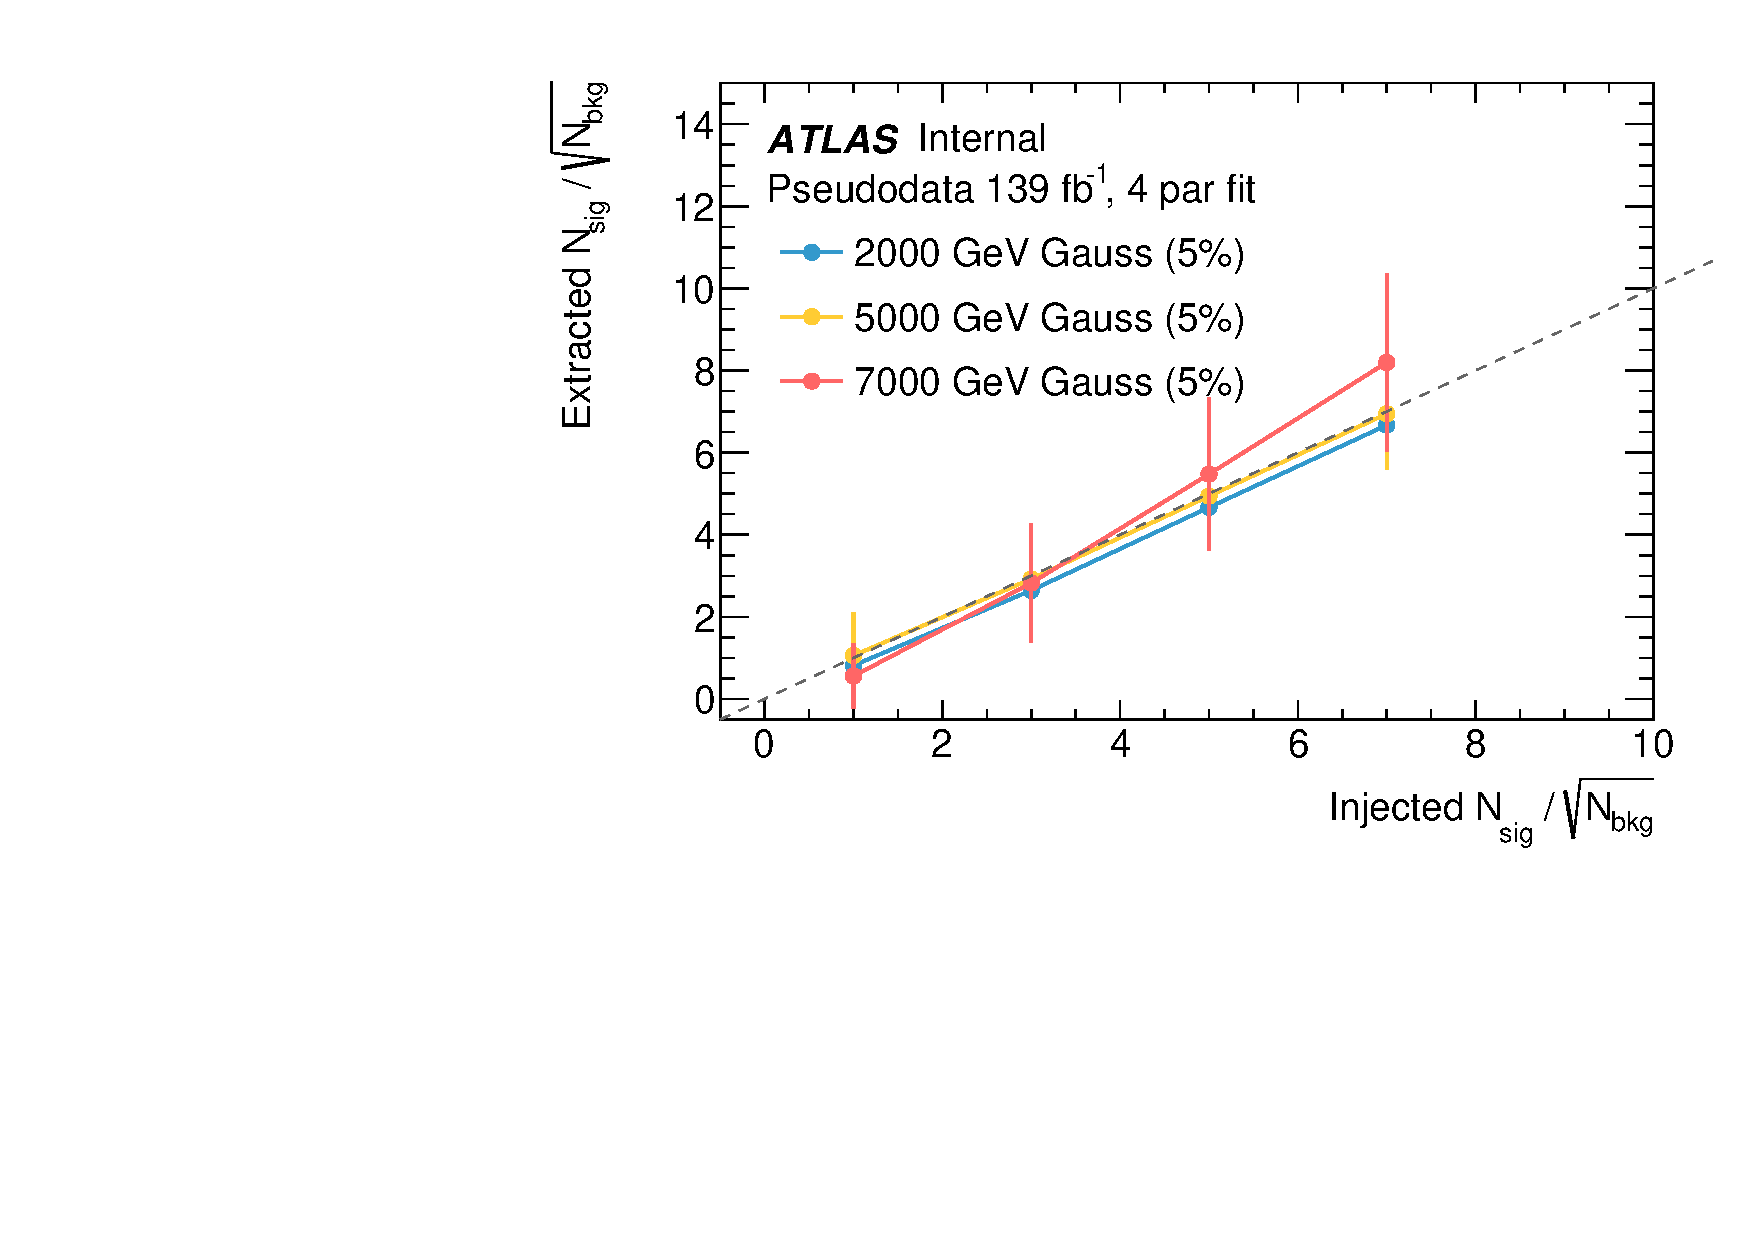
\includegraphics[width=0.35\textwidth]{fig/06-StatisticalFramework/extractionGraphs-1g-5.pdf}}
% %
%\subfloat[] {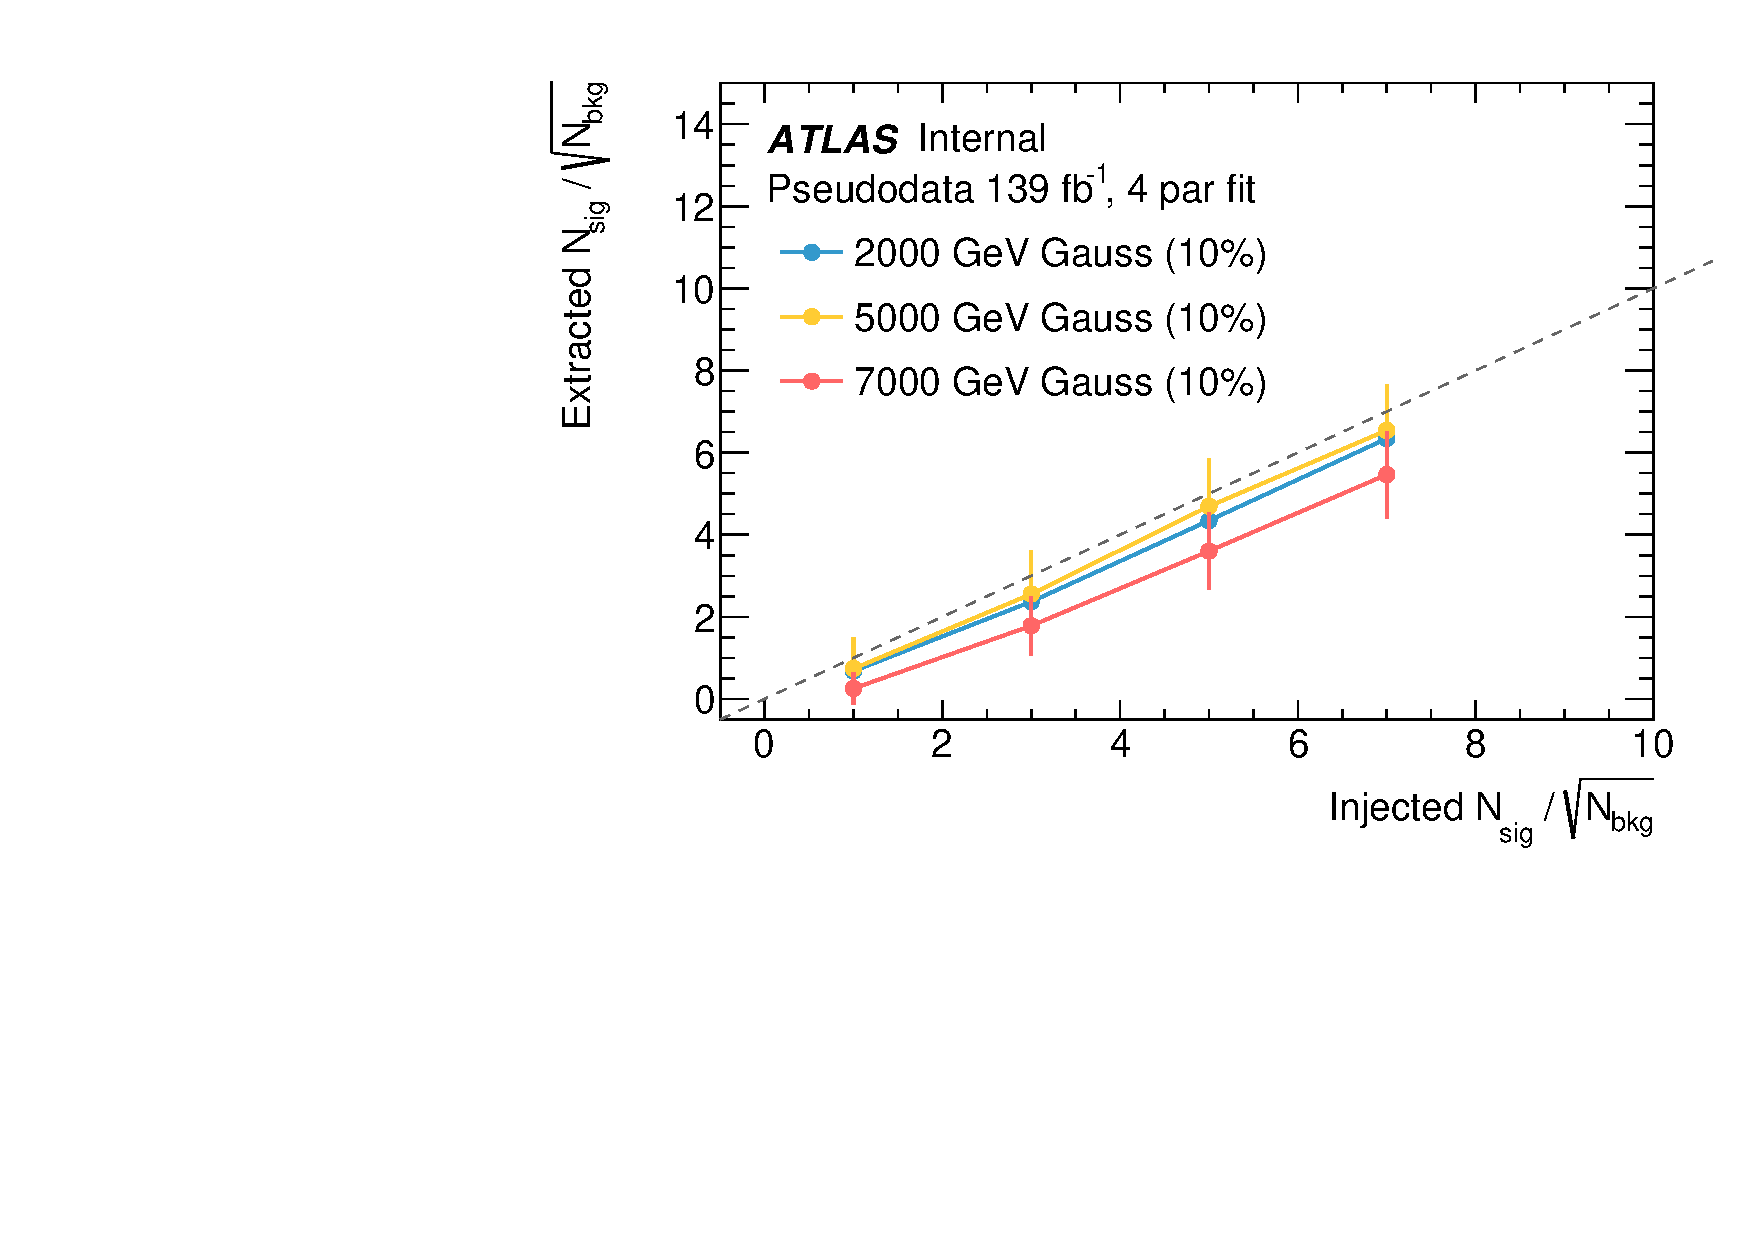
\includegraphics[width=0.35\textwidth]{fig/06-StatisticalFramework/extractionGraphs-1g-10.pdf}}
%\subfloat[] {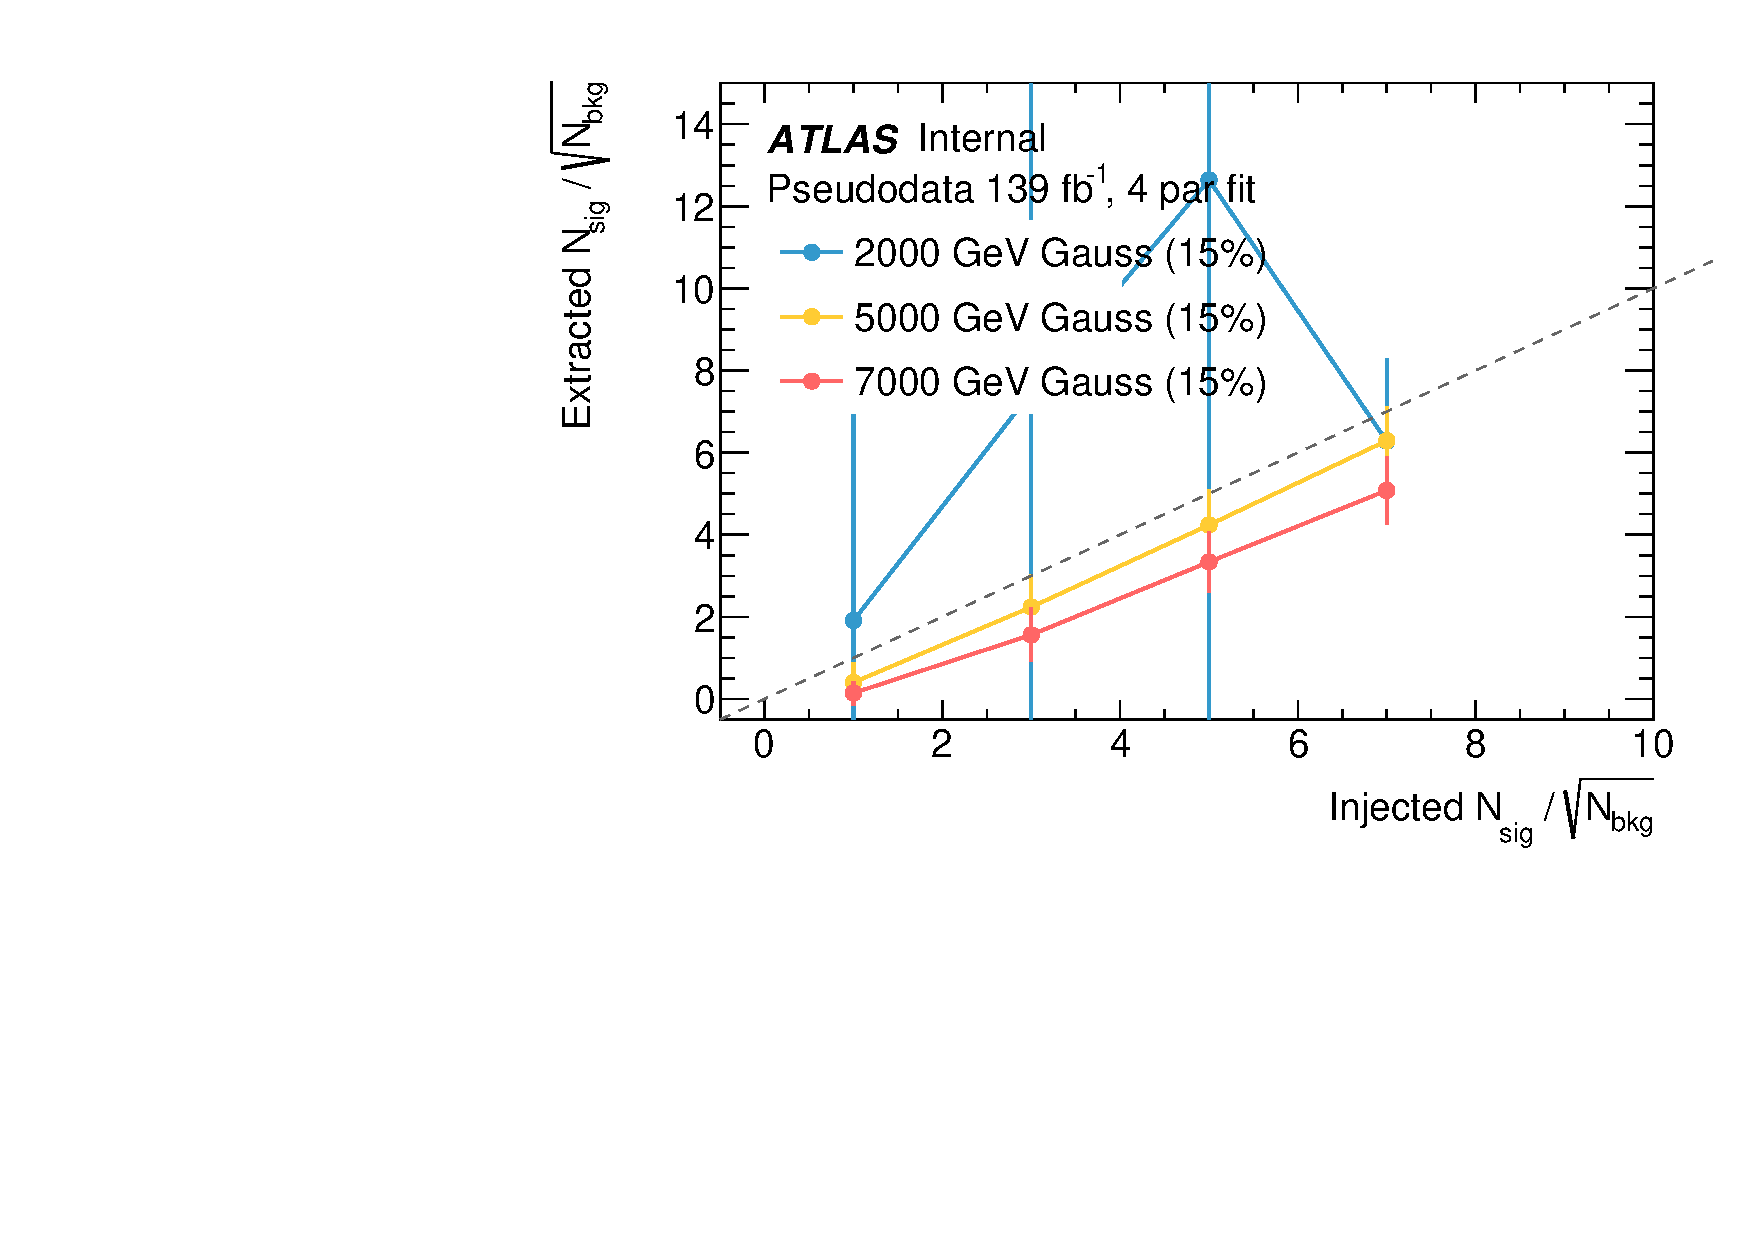
\includegraphics[width=0.35\textwidth]{fig/06-StatisticalFramework/extractionGraphs-1g-15.pdf}}
%\caption{Signal injection tests for the 1 gluon tag category using Gaussian signals of
% (a) 5\% width,
% (b) 10\% width,
% (c) 15\% width. }
% \label{fig:SigInj_1gtag}
%\end{figure}
%
%\begin{figure}[htb]
%\centering
% %
%\subfloat[] {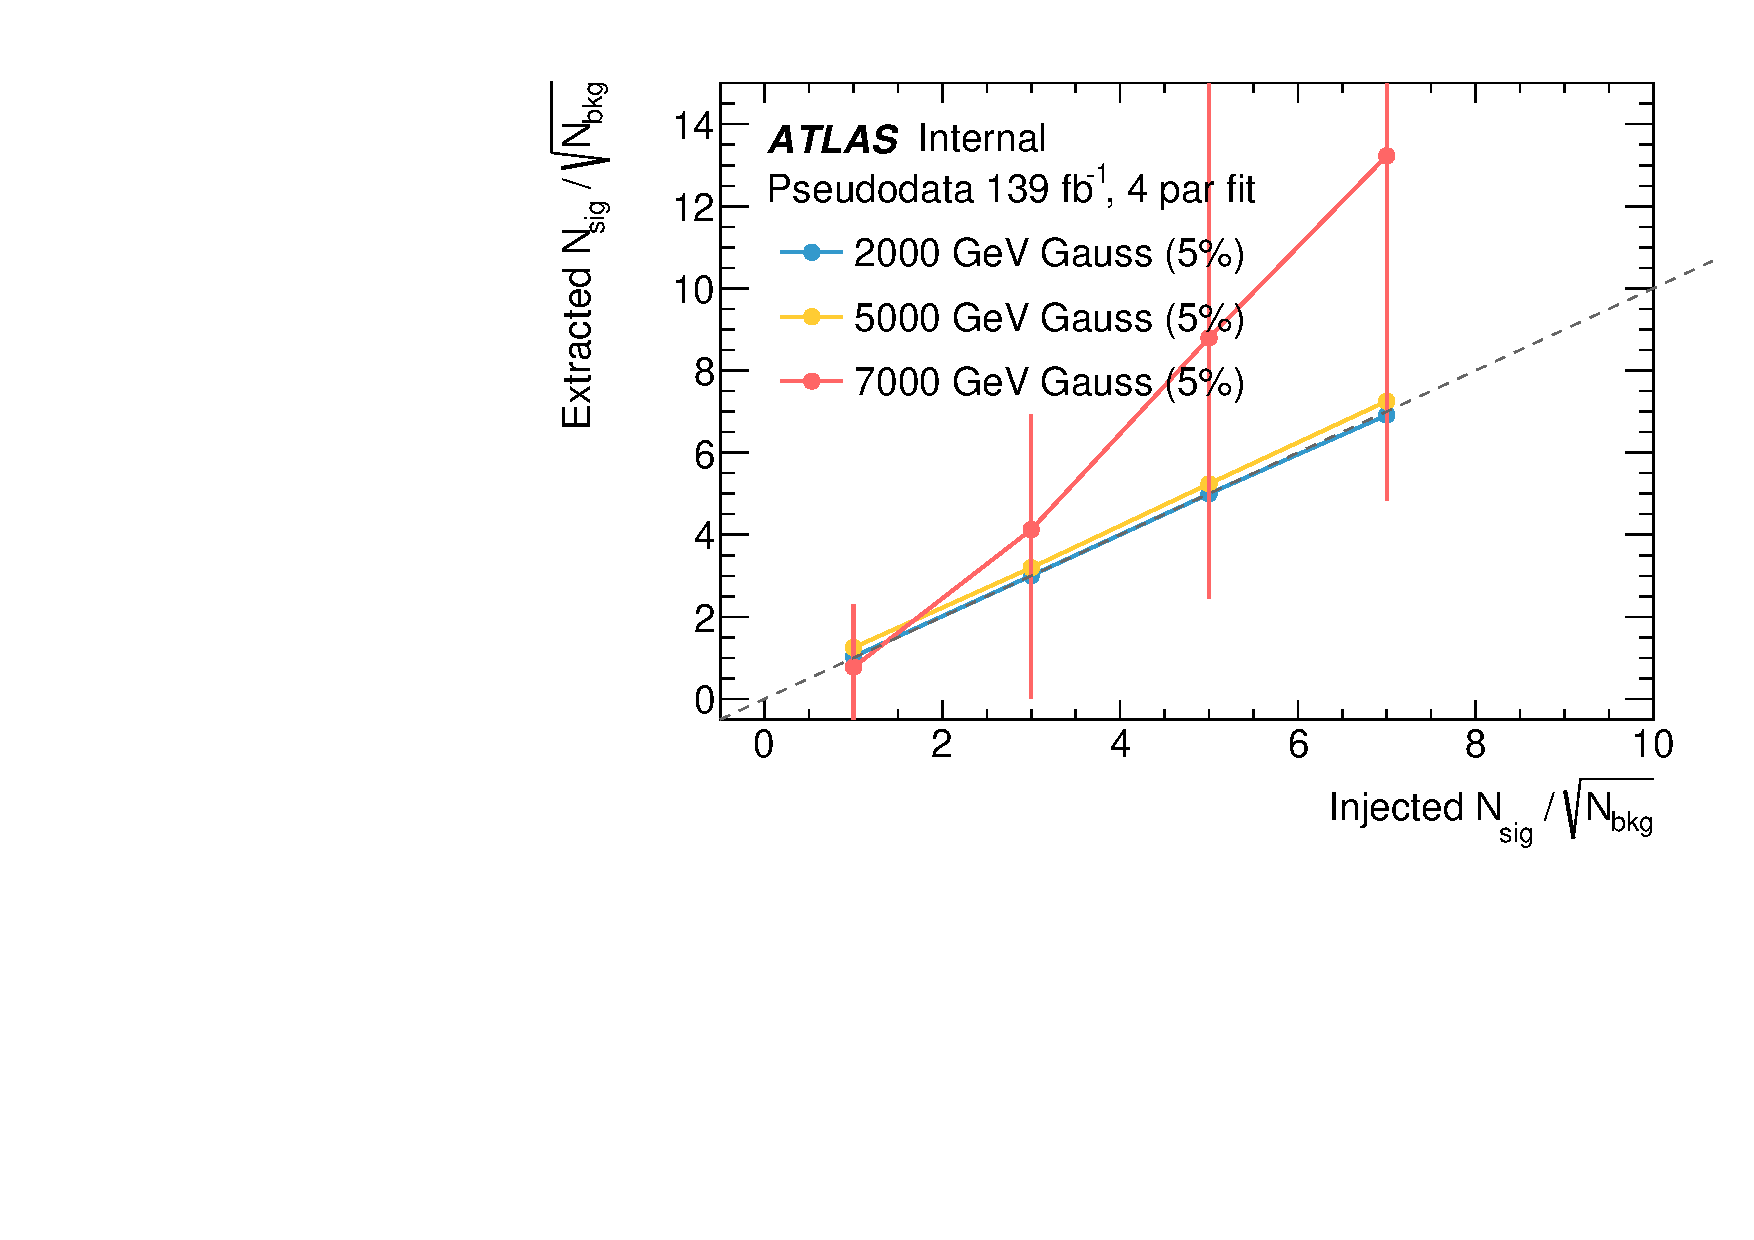
\includegraphics[width=0.35\textwidth]{fig/06-StatisticalFramework/extractionGraphs-2g-5.pdf}}
% %
% \subfloat[] {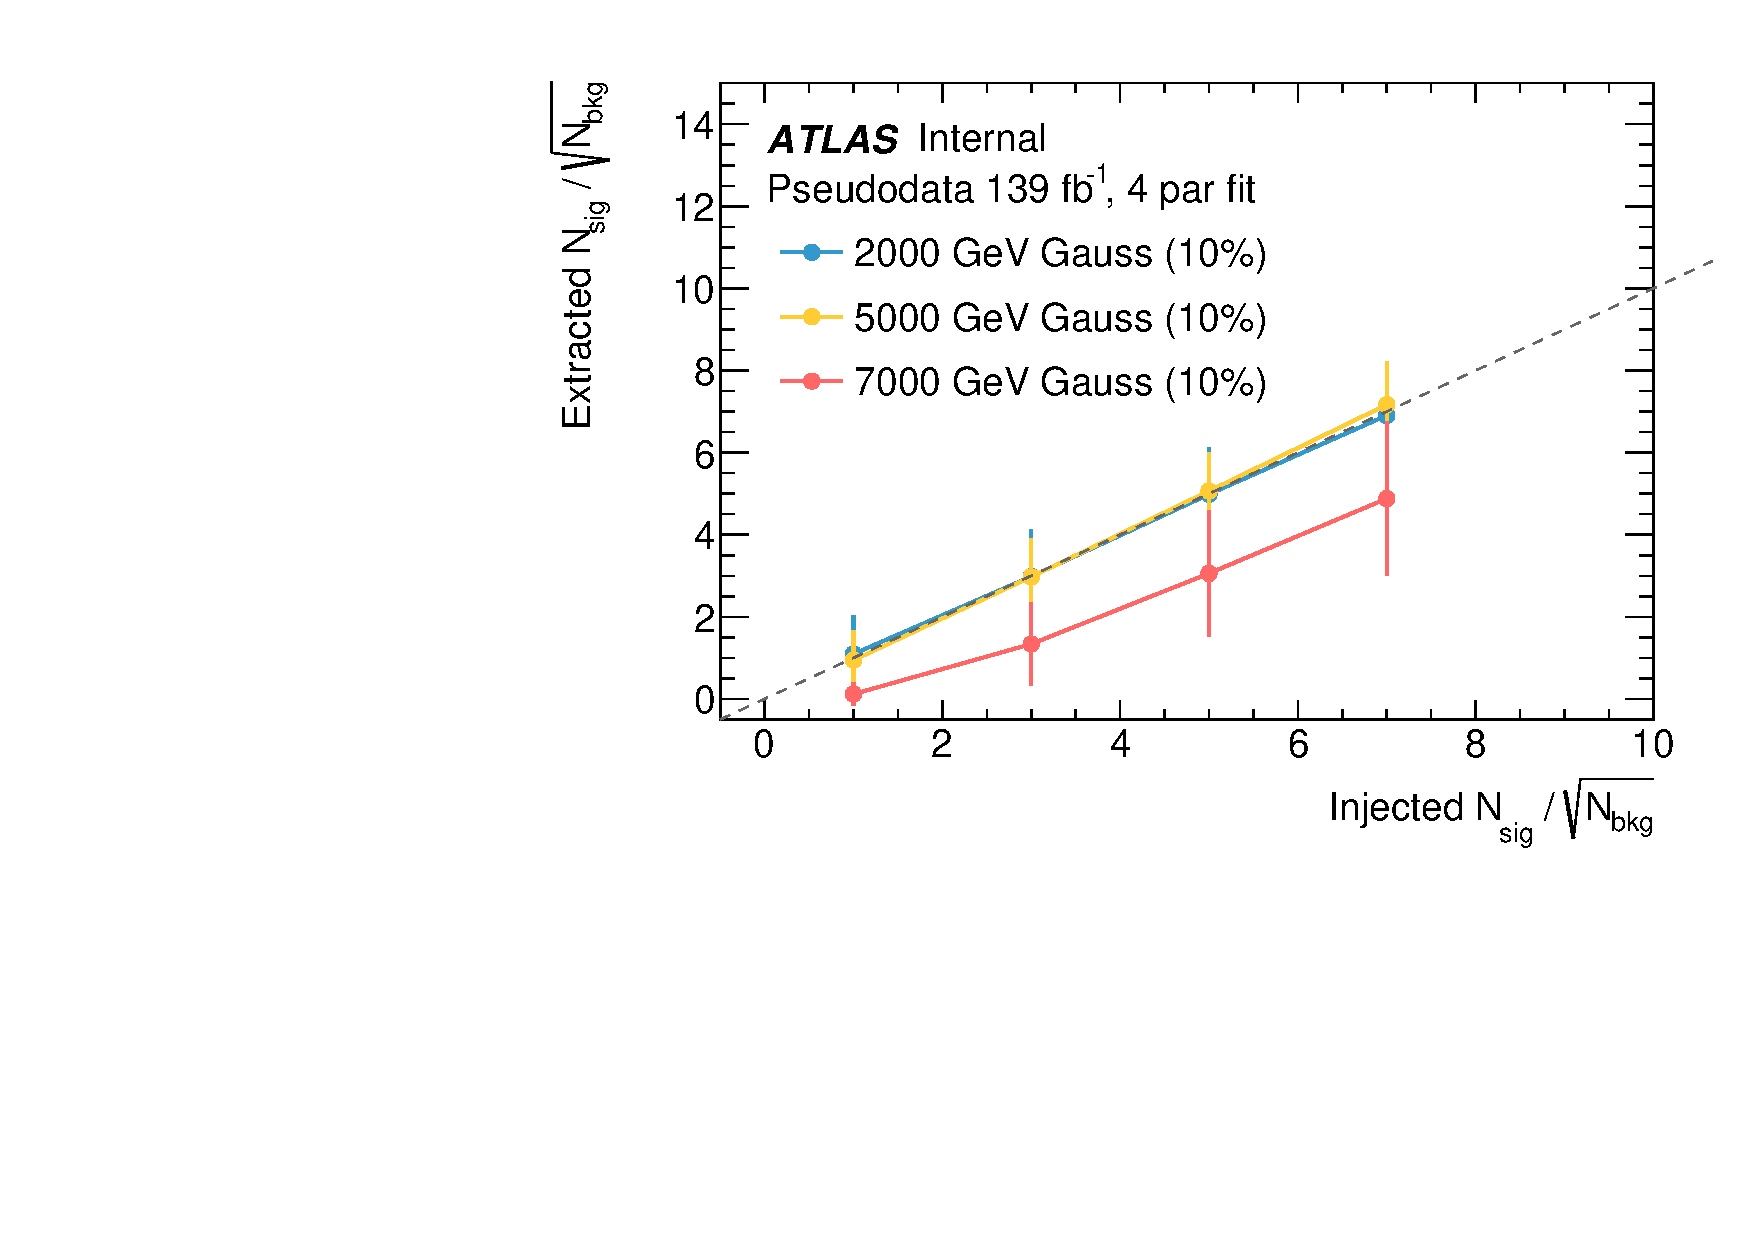
\includegraphics[width=0.35\textwidth]{fig/06-StatisticalFramework/extractionGraphs-2g-10.pdf}}
%\subfloat[] {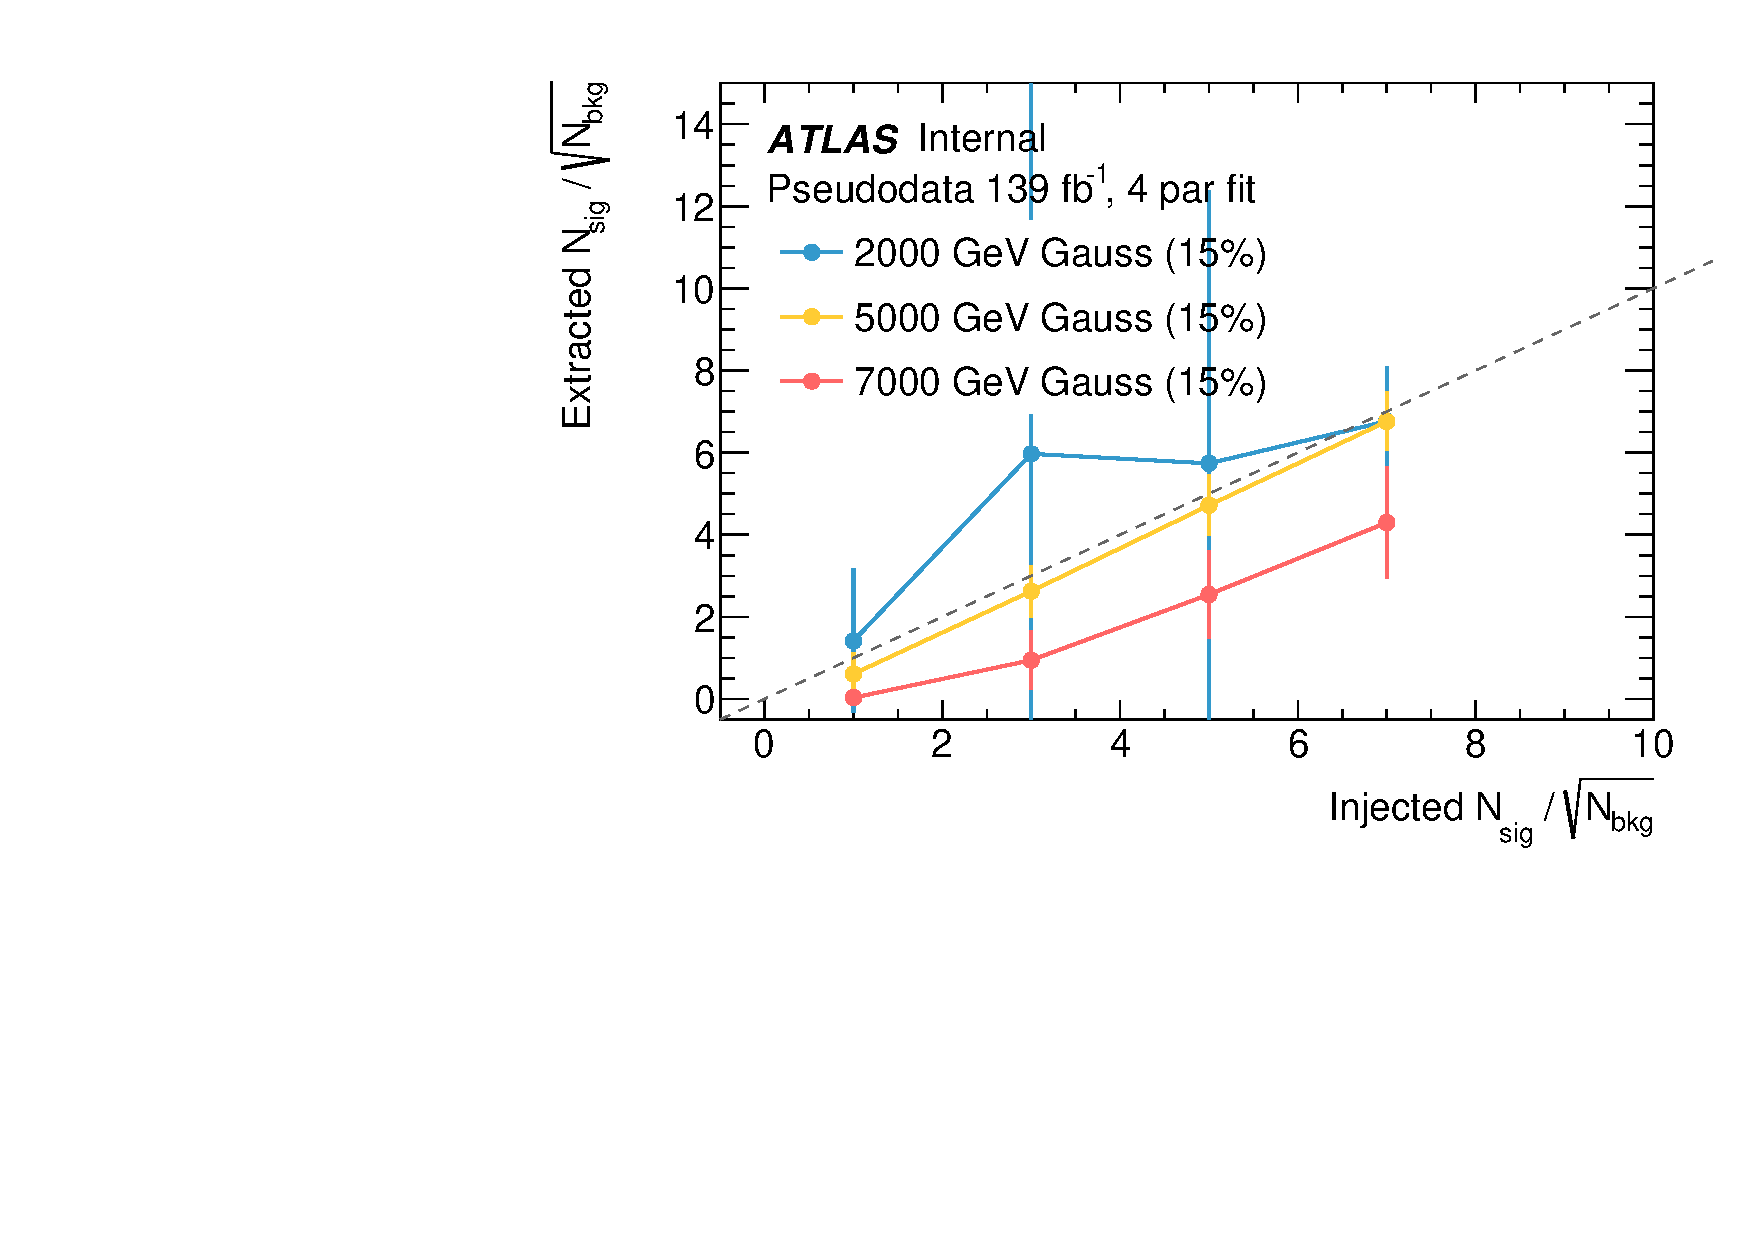
\includegraphics[width=0.35\textwidth]{fig/06-StatisticalFramework/extractionGraphs-2g-15.pdf}}
%\caption{Signal injection tests for the 2 gluon tag category using Gaussian signals of
% (a) 5\% width,
% (b) 10\% width,
% (c) 15\% width. }
% \label{fig:SigInj_2gtag}
%\end{figure}
%
